% Purpose: Assumption-bounded derivations and explanatory diagrams
% for seismic clustering.
% Status: Under Review; mathematical audit incorporated, scientific
% review pending.
% Source-of-truth: doc/UNITS/main/Chapter8_Clustering.tex,
% OGS/src/ogsclustering.py, OGS/test/testogsclustering.py, doc/UNITS/lib.bib
% ==============================================================================
% Document Title: Supplementary Material - Mathematical Derivations for
% Chapter 8:
%                 Seismic Swarm and Density-Based Clustering
% Target Venue / Class: PhD Dissertation Supplementary Material (UniTS / OGS)
% Scientific Objective: Complete step-by-step mathematical derivations,
%                       analytical proofs, asymptotic limits, and physical
%                       constitutive foundations supporting Chapter 8.
% Status: Under Review
% Evidence Anchors: doc/UNITS/main/Chapter8_Clustering.tex,
%                   OGS/src/ogsclustering.py
% ==============================================================================

\providecommand{\bm}[1]{\mathbf{#1}}
\providecommand{\coloneqq}{\mathrel{\mathop:}=}
\providecommand{\mathds}[1]{\mathbb{#1}}
\providecommand{\pak}{\textsc{PAk}}
\providecommand{\kstar}{k^{*}}
\providecommand{\xvec}{\bm{x}}
\providecommand{\mdl}{\mathrm{MDL}}
\providecommand{\Zscore}{Z}
\providecommand{\etas}{\textsc{etas}}

\section*{Mathematical Derivations and Analytical Proofs}
\addcontentsline{toc}{section}{Mathematical Derivations and Analytical Proofs}
\label{sec:supp_clustering}

This supplement supports \cref{chap:clustering} with explicit algebra,
sampling assumptions, and limitations. Exact identities for ideal Poisson
experiments are distinguished from adaptive estimators and phenomenological
physical models. The diagrams are explanatory constructions, not catalogue
measurements or evidence of statistical calibration.

\tikzset{
  clusteringBase/.style={rectangle, rounded corners=2pt, align=center,
  font=\small, inner sep=5pt, minimum height=9mm},
  clusteringTheory/.style={clusteringBase, draw=black!60, dashed, fill=gray!4},
  clusteringImpl/.style={clusteringBase, draw=black!80, line width=0.8pt,
  fill=teal!8},
  clusteringArrow/.style={->, >=Stealth, draw=black!75, line width=0.8pt}
}

% ==============================================================================
% SECTION S1: THE SEISMIC CLUSTERING PROBLEM AND CLASSICAL VALIDITY METRICS
% ==============================================================================
\subsection{Classical Declustering and Cluster Validity Indices}
\label{subsec:supp_classical_metrics}

\paragraph{Derivation of B\r{a}th's Empirical Law (\cref{eq:baths_law}).}
B\r{a}th's law states that the difference in magnitude between a mainshock
and its largest triggered aftershock is approximately constant:
$\Delta m = m_{\mathrm{main}} - m_{\mathrm{after}}^{\max} \approx 1.2$.
The following calculation is an exceedance heuristic, not a derivation of
the empirical value or the mean largest aftershock. Let the expected
number of events
with magnitude $M \ge m$ triggered by a mainshock of magnitude
$m_{\mathrm{main}}$
is modeled by modified aftershock productivity:
\begin{equation}
  \nu(m \mid m_{\mathrm{main}}) = 10^{a + \alpha(m_{\mathrm{main}} -
  m_0) - b(m - m_0)},
  \label{eq:supp_gr_productivity}
\end{equation}
where $a\in\mathbb{R}$, $\alpha,b>0$, and $m_0$ is the completeness
magnitude. Define the characteristic magnitude $m_*$ by unit
expected exceedance:
\begin{equation}
  \nu(m_* \mid m_{\mathrm{main}}) = 1.
  \label{eq:supp_extreme_value_condition}
\end{equation}
Taking the base-10 logarithm of both sides:
\begin{equation}
  a + \alpha(m_{\mathrm{main}} - m_0) - b(m_* - m_0) = 0.
\end{equation}
Assuming self-similarity ($\alpha = b$):
\begin{equation}
  b(m_{\mathrm{main}} - m_*) = -a \implies
  \Delta_* \coloneqq m_{\mathrm{main}} - m_* =
  -\frac{a}{b}.
  \label{eq:supp_baths_ratio}
\end{equation}
More generally, $\Delta_*=[(b-\alpha)(m_{\mathrm{main}}-m_0)-a]/b$.
If exceedance counts are Poisson, then
$\mathbb{P}(M_{\max}\le m)=\exp[-\nu(m\mid m_{\mathrm{main}})]$,
so $m_*$ is an $e^{-1}$ cumulative-probability level, not
$\mathbb{E}[M_{\max}]$. The empirical B\r{a}th value requires independent
catalogue or literature evidence; it is not fixed by this algebra.

\paragraph{Classical Declustering Windows (\cref{eq:classical_window}).}
The deterministic space-time windowing criteria of \citet{gardner1974} and
\citet{reasenberg1985} define interaction envelopes:
\begin{equation}
  \Delta t \le T(M), \qquad \Delta r \le L(M).
\end{equation}
For an ideal circular shear crack of radius $a(M)$, assume the
constitutive relation
$\Delta\sigma_{\mathrm{shear}}$ scales with seismic slip $\bar{D}$ as:
\begin{equation}
  \Delta\sigma_{\mathrm{shear}} = \frac{7\pi}{16}
  \mu_{\mathrm{shear}} \frac{\bar{D}}{a(M)}.
  \label{eq:supp_eshelby_stress}
\end{equation}
The spatial stress perturbation $\Delta\bm{\sigma}(\mathbf{r})$ at
distance $r = \|\mathbf{r}\| \gg a(M)$ decays as a dipolar tensor field:
\begin{equation}
  \|\Delta\bm{\sigma}(\mathbf{r})\| \propto M_0 \, r^{-3}.
  \label{eq:supp_stress_decay}
\end{equation}
For a fixed positive triggering threshold $\Delta\sigma_{\mathrm{crit}}$
and fixed receiver geometry, the far-field scaling yields:
\begin{equation}
  L(M) \propto \left( \frac{M_0(M)}{\Delta\sigma_{\mathrm{crit}}}
  \right)^{\!1/3}
  \propto \bigl( 10^{1.5 M} \bigr)^{1/3} = 10^{0.5 M}.
  \label{eq:supp_spatial_window_scaling}
\end{equation}
This idealized spatial scaling does not reproduce every empirical window.
For $\lambda(t\mid M)=A(M)(t+c)^{-p}$, with $A(M),\mu_0,c,p>0$,
matching the background rate instead gives
\begin{equation}
  T(M)=\max\left\{0,\left[\frac{A(M)}{\mu_0}\right]^{1/p}-c\right\}.
\end{equation}
If $A(M)\propto10^{\alpha M}$, the large-productivity temporal exponent
is $\alpha/p$, not universally $0.5$. The circular-crack coefficient and
its literature attribution remain subject to physical-model review.

\paragraph{Algebraic Decomposition of Classical Validity Indices
(\cref{eq:classical_cvis}).}
Let data points $\mathbf x_i\in\mathbb R^D$, $i=1,\ldots,N$,
be partitioned into $K$ disjoint clusters $C_1,\ldots,C_K$ with cardinalities
$N_k = |C_k|$ and centroids $\mathbf{c}_k = \frac{1}{N_k}\sum_{i \in
C_k} \mathbf{x}_i$.
Let $\bar{\mathbf{x}} = \frac{1}{N}\sum_{i=1}^N \mathbf{x}_i$ denote
the grand mean.
The total scatter matrix $\mathbf{T}$ decomposes uniquely:
\begin{equation}
  \begin{aligned}
    \mathbf{T} &\coloneqq \sum_{i=1}^N (\mathbf{x}_i -
    \bar{\mathbf{x}})(\mathbf{x}_i - \bar{\mathbf{x}})^\top \\
    &= \sum_{k=1}^K \sum_{i \in C_k} \bigl[(\mathbf{x}_i -
    \mathbf{c}_k) + (\mathbf{c}_k - \bar{\mathbf{x}})\bigr]
    \bigl[(\mathbf{x}_i - \mathbf{c}_k) + (\mathbf{c}_k -
    \bar{\mathbf{x}})\bigr]^\top \\
    &= \sum_{k=1}^K \sum_{i \in C_k} (\mathbf{x}_i -
    \mathbf{c}_k)(\mathbf{x}_i - \mathbf{c}_k)^\top
    + \sum_{k=1}^K N_k (\mathbf{c}_k -
    \bar{\mathbf{x}})(\mathbf{c}_k - \bar{\mathbf{x}})^\top \\
    &\quad + \sum_{k=1}^K \left[
      \mathbf{a}_k(\mathbf{c}_k-\bar{\mathbf{x}})^\top
    +(\mathbf{c}_k-\bar{\mathbf{x}})\mathbf{a}_k^\top\right] \\
    &= \mathbf{W} + \mathbf{B},
  \end{aligned}
  \label{eq:supp_scatter_decomposition}
\end{equation}
where $\mathbf{a}_k=\sum_{i\in C_k}(\mathbf{x}_i-\mathbf{c}_k)=\mathbf{0}$,
$\mathbf{W}$ is the within-cluster scatter matrix and $\mathbf{B}$ is the
between-cluster scatter matrix. Taking the matrix trace:
\begin{equation}
  \mathrm{Tr}(\mathbf{W}) = \sum_{k=1}^K \sum_{i \in C_k}
  \|\mathbf{x}_i - \mathbf{c}_k\|^2, \qquad
  \mathrm{Tr}(\mathbf{B}) = \sum_{k=1}^K N_k \|\mathbf{c}_k -
  \bar{\mathbf{x}}\|^2.
\end{equation}
The \acf{CH} is the normalized ratio of explained to unexplained variance:
\begin{equation}
  \mathrm{CH} = \frac{\mathrm{Tr}(\mathbf{B}) / (K -
  1)}{\mathrm{Tr}(\mathbf{W}) / (N - K)}.
\end{equation}
Assume $2\le K<N$ and nonzero within-cluster scatter. A non-convex
support can have an off-support centroid, making centroid scatter a poor
description of its geometry. Non-convexity alone neither forces this
configuration nor implies $\mathrm{CH}\to0$.

Similarly, the \acf{DB} evaluates cluster dispersion:
\begin{equation}
  s_k \coloneqq \frac{1}{N_k}\sum_{i \in C_k} \|\mathbf{x}_i
  - \mathbf{c}_k\|, \qquad
  R_{kl} \coloneqq \frac{s_k + s_l}{\|\mathbf{c}_k - \mathbf{c}_l\|}, \qquad
  \mathrm{DB} \coloneqq \frac{1}{K}\sum_{k=1}^K \max_{l \ne k} R_{kl}.
\end{equation}
If two interleaved curved clusters wrap around each other, their centroids
$\mathbf{c}_k$ and $\mathbf{c}_l$ can be nearly coincident
($\|\mathbf{c}_k - \mathbf{c}_l\| \to 0$)
despite a wide density void between them, causing $R_{kl} \to \infty$ and
penalizing the partition in the nondegenerate limit. The mean-distance
definition matches the scikit-learn wrapper; exact coincident-centroid
cases require the library's numerical conventions.

% ==============================================================================
% SECTION S2: MEASURE-THEORETIC STOCHASTIC POINT PROCESSES
% ==============================================================================
\subsection{Stochastic Point Process Foundations and PELT Segmentation}
\label{subsec:supp_point_processes}

\paragraph{Derivation of the Inhomogeneous Poisson Count
Distribution (\cref{eq:poisson_count_dist}).}
Let $A \in \mathcal{B}([0, T_{\mathrm{obs}}])$ be a Borel set with cumulative
intensity $\Lambda(A) = \int_A \lambda(t)\,\mathrm{d}t < \infty$. Partition $A$
into $M$ disjoint subsets $A_1, \dots, A_M$ such that $\Lambda(A_m)
= \Lambda(A)/M$.
Assume independent increments and uniform infinitesimal probabilities
across the partition, with the remainders below uniform in $m$:
\begin{equation}
  p_M \coloneqq \mathbb{P}\bigl(N(A_m) = 1\bigr) =
  \frac{\Lambda(A)}{M} + o\left(\frac{1}{M}\right), \qquad
  \mathbb{P}\bigl(N(A_m) \ge 2\bigr) = o\left(\frac{1}{M}\right).
\end{equation}
The probability of any multiple-count cell is $M\,o(M^{-1})=o(1)$.
The total count $N(A) = \sum_{m=1}^M
N(A_m)$ converges
to a sum of independent Bernoulli trials. For any $k \in \mathbb{N}_0$:
\begin{equation}
  \begin{aligned}
    \mathbb{P}\bigl(N(A) = k\bigr)
    &= \lim_{M \to \infty} \binom{M}{k} p_M^k (1 - p_M)^{M - k} \\
    &= \lim_{M \to \infty} \frac{M(M-1)\cdots(M-k+1)}{k!} \left(
    \frac{\Lambda(A)}{M} \right)^{\!k} \left( 1 -
    \frac{\Lambda(A)}{M} \right)^{\!M - k} \\
    &= \frac{\Lambda(A)^k}{k!} \lim_{M \to \infty} \left[
    \prod_{j=0}^{k-1}\left(1 - \frac{j}{M}\right) \right] \left( 1 -
    \frac{\Lambda(A)}{M} \right)^{\!M} \left( 1 -
    \frac{\Lambda(A)}{M} \right)^{\!-k} \\
    &= \frac{\Lambda(A)^k}{k!} \cdot 1 \cdot e^{-\Lambda(A)} \cdot 1
    = \frac{\Lambda(A)^k}{k!} e^{-\Lambda(A)},
  \end{aligned}
  \label{eq:supp_poisson_limit}
\end{equation}
establishing the exact Poisson count distribution in
\cref{eq:poisson_count_dist}.

\paragraph{Derivation of Campbell's Theorem and Moments
(\cref{eq:campbell_mean_var,eq:campbell_char_fn}).}
Let $g: [0, T_{\mathrm{obs}}] \to \mathbb{R}$ be bounded and
measurable. Define the
random sum $S_g \coloneqq \int_0^{T_{\mathrm{obs}}}
g(t)\,N(\mathrm{d}t) = \sum_{i=1}^{N(T_{\mathrm{obs}})} g(t_i)$.
Let $g_M=\sum_{m=1}^{J_M}a_{M,m}\mathbf{1}_{A_{M,m}}$ be bounded
simple functions on disjoint measurable sets, converging pointwise to $g$.
With finite intensity measure, define:
\begin{equation}
  S_g^{(M)} = \sum_{m=1}^{J_M} a_{M,m} N(A_{M,m}).
\end{equation}
Taking the expectation:
\begin{equation}
  \mathbb{E}\bigl[S_g^{(M)}\bigr]
  =\sum_{m=1}^{J_M}a_{M,m}\Lambda(A_{M,m})
  =\int g_M(t)\lambda(t)\,\mathrm{d}t.
\end{equation}
Bounded convergence gives the mean; convergence in $L^2$ of the random
integrals gives the variance, since $N(T_{\mathrm{obs}})$ has finite
second moment:
\begin{equation}
  \mathbb{E}[S_g] = \int_0^{T_{\mathrm{obs}}} g(t)\lambda(t)\,\mathrm{d}t.
  \label{eq:supp_campbell_mean}
\end{equation}
Because counts on the $A_{M,m}$ are mutually independent:
\begin{equation}
  \Var\bigl(S_g^{(M)}\bigr)
  =\sum_{m=1}^{J_M}a_{M,m}^2\Lambda(A_{M,m})
  =\int g_M(t)^2\lambda(t)\,\mathrm{d}t,
\end{equation}
which converges as $M \to \infty$ to:
\begin{equation}
  \Var(S_g) = \int_0^{T_{\mathrm{obs}}} g^2(t)\lambda(t)\,\mathrm{d}t.
  \label{eq:supp_campbell_var}
\end{equation}
For the characteristic functional, evaluate the expectation of the product:
\begin{equation}
  \begin{aligned}
    \mathbb{E}\bigl[\exp(\mathrm{i}\theta S_g)\bigr]
    &= \lim_{M \to \infty} \prod_{m=1}^{J_M}
    \mathbb{E}\left[e^{\mathrm{i}\theta a_{M,m}N(A_{M,m})}\right] \\
    &= \lim_{M \to \infty}\exp\left[
    \sum_{m=1}^{J_M}\Lambda(A_{M,m})(e^{\mathrm{i}\theta a_{M,m}}-1)\right] \\
    &= \lim_{M \to \infty}\exp\left[
    \int(e^{\mathrm{i}\theta g_M(t)}-1)\lambda(t)\,\mathrm{d}t\right] \\
    &= \exp\left( \int_0^{T_{\mathrm{obs}}}
    \bigl(e^{\mathrm{i}\theta g(t)} - 1\bigr)\lambda(t)\,\mathrm{d}t \right),
  \end{aligned}
  \label{eq:supp_char_functional}
\end{equation}
completing the proof of \cref{thm:campbell}.

\paragraph{Derivation of the Continuous Point-Process Likelihood
(\cref{eq:ipp_likelihood,eq:ipp_log_likelihood}).}
Let observed event times be $0 < t_1 < t_2 < \dots < t_N < T_{\mathrm{obs}}$.
Partition $[0, T_{\mathrm{obs}}]$ into $M$ bins $I_m = [s_{m-1},
s_m)$ of width $\Delta = T_{\mathrm{obs}}/M$.
For sufficiently large $M$, each bin contains at most one event.
Let $\mathcal{I}_{\mathrm{event}} = \{m : N(I_m) = 1\}$ with
$|\mathcal{I}_{\mathrm{event}}| = N$,
and $\mathcal{I}_{\mathrm{empty}} = \{m : N(I_m) = 0\}$.
The joint probability is:
\begin{equation}
  \mathbb{P}\bigl(\{N(I_m)\}_{m=1}^M\bigr) = \prod_{m \in
  \mathcal{I}_{\mathrm{event}}} \bigl[\Lambda(I_m)
  e^{-\Lambda(I_m)}\bigr] \prod_{m \in \mathcal{I}_{\mathrm{empty}}}
  e^{-\Lambda(I_m)}.
\end{equation}
Combining the exponential terms:
\begin{equation}
  \prod_{m=1}^M e^{-\Lambda(I_m)} = \exp\left( -\sum_{m=1}^M
  \Lambda(I_m) \right) = \exp\left( -\int_0^{T_{\mathrm{obs}}}
  \lambda(s)\,\mathrm{d}s \right).
\end{equation}
For this bin-limit proof, assume $\lambda$ is continuous and positive at
each observed $t_i\in I_m$; then:
\begin{equation}
  \Lambda(I_m) = \int_{I_m} \lambda(s)\,\mathrm{d}s =
  \lambda(t_i)\Delta + o(\Delta).
\end{equation}
Substituting back:
\begin{equation}
  \mathbb{P}\bigl(\{N(I_m)\}_{m=1}^M\bigr) = \left( \prod_{i=1}^N
  \bigl[\lambda(t_i)\Delta + o(\Delta)\bigr] \right) \exp\left(
  -\int_0^{T_{\mathrm{obs}}} \lambda(s)\,\mathrm{d}s \right).
\end{equation}
Dividing by the reference Lebesgue measure $\Delta^N$ and taking
$\Delta \to 0^+$:
\begin{equation}
  \mathcal{L}(\lambda) = \lim_{\Delta \to 0^+}
  \frac{\mathbb{P}(\{N(I_m)\})}{\Delta^N} = \left( \prod_{i=1}^N
  \lambda(t_i) \right) \exp\left( -\int_0^{T_{\mathrm{obs}}}
  \lambda(s)\,\mathrm{d}s \right).
\end{equation}
Taking the natural logarithm:
\begin{equation}
  \ell(\lambda) = \ln \mathcal{L}(\lambda) = \sum_{i=1}^N \ln
  \lambda(t_i) - \int_0^{T_{\mathrm{obs}}} \lambda(s)\,\mathrm{d}s,
\end{equation}
which is \cref{eq:ipp_log_likelihood}, using a fixed time unit.
Relative to a Poisson reference law $Q$ with positive rate $q(t)$,
the exact likelihood ratio is instead
\begin{equation}
  \ln\frac{\mathrm{d}P_\lambda}{\mathrm{d}Q}
  =\int\ln\frac{\lambda(t)}{q(t)}\,N(\mathrm{d}t)
  -\int[\lambda(t)-q(t)]\,\mathrm{d}t.
\end{equation}
The difference is parameter-independent for fixed $q$.

\paragraph{Maximum Entropy Derivation of the IPP
(\cref{eq:max_entropy_bound}).}
Let $\mathcal{P}$ be the set of probability distributions $P$ over
point trajectories
on $[0, T_{\mathrm{obs}}]$, absolutely continuous with respect to the
Poisson reference law $\mathbb{Q}$ of positive deterministic rate $q(t)$.
Assume finite relative entropies and integrability of
$\lambda|\ln(\lambda/q)|$. The negative relative entropy is:
\begin{equation}
  h(P \parallel \mathbb{Q}) = -\int
  \frac{\mathrm{d}P}{\mathrm{d}\mathbb{Q}}(\omega) \ln\left(
  \frac{\mathrm{d}P}{\mathrm{d}\mathbb{Q}}(\omega) \right)
  \mathrm{d}\mathbb{Q}(\omega).
\end{equation}
We maximize $h(P \parallel \mathbb{Q})$ subject to the moment constraint:
\begin{equation}
  \mathbb{E}_P[N(A)] = \int_A \lambda(t)\,\mathrm{d}t, \qquad
  \forall A \in \mathcal{B}([0, T_{\mathrm{obs}}]),
\end{equation}
and probability normalization $\int \mathrm{d}P = 1$. The Lagrangian
functional is:
\begin{equation}
  \mathcal{J}[p] = -\int p(\omega)\ln
  p(\omega)\,\mathrm{d}\mathbb{Q}(\omega) - \alpha_0 \left(\int
  p(\omega)\,\mathrm{d}\mathbb{Q}(\omega) - 1\right) -
  \int_0^{T_{\mathrm{obs}}}
  \beta(t)\left(\mathbb{E}_P[\mathrm{d}N(t)] - \lambda(t)\,\mathrm{d}t\right).
\end{equation}
Taking the functional derivative with respect to density $p(\omega)$
and setting to zero:
\begin{equation}
  \frac{\delta\mathcal{J}}{\delta p(\omega)} = -\ln p(\omega) - 1 -
  \alpha_0 - \int_0^{T_{\mathrm{obs}}} \beta(t)\,N(\mathrm{d}t; \omega) = 0.
\end{equation}
Solving for $p(\omega)$:
\begin{equation}
  p(\omega) = \frac{1}{\mathcal{Z}} \exp\left(
  -\int_0^{T_{\mathrm{obs}}} \beta(t)\,N(\mathrm{d}t; \omega) \right).
\end{equation}
Matching the constraint requires $\beta(t)=-\ln[\lambda(t)/q(t)]$.
More rigorously, the fixed mean measure implies
\begin{equation}
  D(P\parallel\mathbb{Q})
  =D(P\parallel P_\lambda)+D(P_\lambda\parallel\mathbb{Q}),
\end{equation}
because the expectation under $P$ of
$\ln(\mathrm{d}P_\lambda/\mathrm{d}\mathbb{Q})$
depends only on that mean measure. Nonnegativity of relative entropy gives
the unique optimum $P=P_\lambda$, under the stated finiteness assumptions.

\paragraph{Statistical Mechanics Grand Canonical Isomorphism
(\cref{eq:fugacity_def,eq:stat_mech_likelihood_equiv}).}
Consider an ideal one-dimensional gas of non-interacting classical
particles with
spatial coordinates $t_i \in [0, T_{\mathrm{obs}}]$. In statistical
thermodynamics
with temperature $\beta_{\mathrm{therm}} =
1/(k_{\mathrm{B}}\mathcal{T}) = 1$, the
grand partition function is:
\begin{equation}
  \Xi = \sum_{N=0}^\infty \frac{1}{N!} \prod_{i=1}^N \left(
  \int_0^{T_{\mathrm{obs}}} \lambda_0 z(t_i)\,\mathrm{d}t_i \right)
  = \sum_{N=0}^\infty \frac{1}{N!} \left( \int_0^{T_{\mathrm{obs}}}
  \lambda_0 z(t)\,\mathrm{d}t \right)^{\!N}.
\end{equation}
Using the Taylor series of the exponential $\sum_{N=0}^\infty x^N / N! = e^x$:
\begin{equation}
  \Xi = \exp\left( \int_0^{T_{\mathrm{obs}}} \lambda_0
  z(t)\,\mathrm{d}t \right).
  \label{eq:supp_grand_partition_eval}
\end{equation}
Here $\lambda_0>0$ is a reference rate, and the dimensionless activity
is $z(t)=\lambda(t)/\lambda_0$. This yields $\Xi =
\exp(\Lambda([0, T_{\mathrm{obs}}]))$.
The grand thermodynamic potential is defined as:
\begin{equation}
  \Omega_{\mathrm{grand}} \coloneqq -\ln \Xi =
  -\int_0^{T_{\mathrm{obs}}} \lambda(t)\,\mathrm{d}t.
\end{equation}
In thermal units, the chemical potential is
$\mu_{\mathrm{chem}}(t)=\ln z(t)$; its negative is an effective potential.
Rewriting the point-process log-likelihood:
\begin{equation}
  \begin{aligned}
    \ell(\lambda)-N\ln\lambda_0 &= \sum_{i=1}^N \ln z(t_i) -
    \int_0^{T_{\mathrm{obs}}} \lambda(s)\,\mathrm{d}s \\
    &= \sum_{i=1}^N \mu_{\mathrm{chem}}(t_i) +
    \Omega_{\mathrm{grand}} \equiv -\mathcal{F}_{\mathrm{stat}}[\lambda],
  \end{aligned}
\end{equation}
This ideal-gas representation is algebraic. Maximum likelihood minimizes
the full negative log-likelihood, not the grand potential alone, and does
not identify a physical temperature for earthquake occurrence.

\paragraph{Piecewise-Constant MLE and Profile Log-Likelihood
(\cref{eq:piecewise_loglik,eq:profile_loglik}).}
For partition $0 = \tau_0 < \dots < \tau_{K+1} = T_{\mathrm{obs}}$ with rate
$\lambda(t) = \lambda_j$ on $I_j = (\tau_j, \tau_{j+1}]$ of length $\Delta_j$:
\begin{equation}
  \int_0^{T_{\mathrm{obs}}} \lambda(s)\,\mathrm{d}s = \sum_{j=0}^K
  \int_{\tau_j}^{\tau_{j+1}} \lambda_j\,\mathrm{d}s = \sum_{j=0}^K
  \lambda_j \Delta_j.
\end{equation}
Similarly:
\begin{equation}
  \sum_{i=1}^N \ln\lambda(t_i) = \sum_{j=0}^K \sum_{i: t_i \in I_j}
  \ln\lambda_j = \sum_{j=0}^K n_j \ln\lambda_j.
\end{equation}
Combining these yields \cref{eq:piecewise_loglik}:
\begin{equation}
  \ell(\{\lambda_j\}) = \sum_{j=0}^K \bigl[ n_j \ln\lambda_j -
  \lambda_j \Delta_j \bigr].
\end{equation}
Taking the partial derivative with respect to $\lambda_j$:
\begin{equation}
  \frac{\partial \ell}{\partial \lambda_j} = \frac{n_j}{\lambda_j} -
  \Delta_j = 0 \implies \hat{\lambda}_j = \frac{n_j}{\Delta_j}.
\end{equation}
The second derivative is strictly negative:
\begin{equation}
  \frac{\partial^2 \ell}{\partial \lambda_j^2} =
  -\frac{n_j}{\lambda_j^2} < 0, \qquad (\forall n_j > 0),
\end{equation}
guaranteeing an interior maximum for $n_j>0$. For an empty segment,
the maximum is $\hat\lambda_j=0$ if zero rates are admissible; otherwise
only a supremum is attained as $\lambda_j\downarrow0$.
Substituting $\hat{\lambda}_j
= n_j/\Delta_j$ back:
\begin{equation}
  \ell_{\mathrm{profile}}(\{\tau_j\}) = \sum_{j=0}^K \left[ n_j
    \ln\left(\frac{n_j}{\Delta_j}\right) -
  \left(\frac{n_j}{\Delta_j}\right)\Delta_j \right]
  = \sum_{j=0}^K \left[ n_j \ln\left(\frac{n_j}{\Delta_j}\right) - n_j \right],
\end{equation}
which is \cref{eq:profile_loglik}, with $0\ln0=0$. A fixed candidate
grid or minimum segment duration is needed to exclude arbitrarily narrow
event-containing intervals in changepoint optimization.

\paragraph{Proof of the PELT Pruning Theorem
(\cref{eq:pelt_bellman,eq:pelt_pruning_rule}).}
Let $F(s)$ denote the minimum penalized cost for data on $[0, t_s]$.
Bellman's principle states:
\begin{equation}
  F(s) = \min_{0 \le v < s} \bigl[ F(v) + \mathcal{C}((t_v, t_s]) +
  \beta \bigr].
\end{equation}
Assume there exists $K_{\mathrm{prune}} \ge 0$ such that for all $v < s < u$:
\begin{equation}
  \mathcal{C}((t_v, t_s]) + \mathcal{C}((t_s, t_u]) +
  K_{\mathrm{prune}} \le \mathcal{C}((t_v, t_u]).
  \label{eq:supp_pelt_subadditivity}
\end{equation}
Suppose candidate $v$ satisfies the pruning condition at step $s$:
\begin{equation}
  F(v) + \mathcal{C}((t_v, t_s]) + K_{\mathrm{prune}} \ge F(s).
  \label{eq:supp_pruning_hyp}
\end{equation}
We must show that an alternative through $s$ is no worse at any admissible
future time $u>s$:
\begin{equation}
  F(v) + \mathcal{C}((t_v, t_u]) + \beta \ge F(u).
\end{equation}
Using the subadditivity condition in \cref{eq:supp_pelt_subadditivity}:
\begin{equation}
  \begin{aligned}
    F(v) + \mathcal{C}((t_v, t_u]) + \beta
    &\ge F(v) + \mathcal{C}((t_v, t_s]) + \mathcal{C}((t_s, t_u]) +
    K_{\mathrm{prune}} + \beta \\
    &= \bigl[ F(v) + \mathcal{C}((t_v, t_s]) + K_{\mathrm{prune}}
    \bigr] + \mathcal{C}((t_s, t_u]) + \beta \\
    &\ge F(s) + \mathcal{C}((t_s, t_u]) + \beta \quad \text{(by
    \cref{eq:supp_pruning_hyp})} \\
    &\ge \min_{0 \le w < u} \bigl[ F(w) + \mathcal{C}((t_w, t_u]) +
    \beta \bigr] = F(u).
  \end{aligned}
\end{equation}
Hence $v$ can be discarded without losing the optimum value, although tied
optimal partitions may be removed. This proof establishes exact pruning,
not its expected running time. Expected $\mathcal{O}(N)$ requires the
additional cost and stochastic assumptions of \citet{killick2012}; the
worst case remains quadratic. Any minimum-length constraints must also
preserve feasibility of the dominating alternative.

% ==============================================================================
% SECTION S3: INTRINSIC DIMENSION AND POINT-ADAPTIVE DENSITY ESTIMATION
% ==============================================================================
\subsection{TWO-NN Intrinsic Dimension and PAk Density Estimation}
\label{subsec:supp_pak_derivations}

\paragraph{Volume of the Unit $d$-Ball (\cref{eq:unit_ball_volume}).}
Consider the $d$-dimensional Gaussian integral evaluated in
Cartesian coordinates:
\begin{equation}
  I_d \coloneqq \int_{\mathbb{R}^d} \exp\left(-\sum_{i=1}^d
  x_i^2\right) \mathrm{d}x_1 \cdots \mathrm{d}x_d
  = \prod_{i=1}^d \left( \int_{-\infty}^\infty
  e^{-x_i^2}\,\mathrm{d}x_i \right) = \bigl(\sqrt{\pi}\bigr)^d = \pi^{d/2}.
\end{equation}
Transforming to spherical coordinates with radial coordinate $r =
\|\mathbf{x}\|$ and
surface area element of the unit sphere $\mathrm{d}\Omega_{d-1}$:
\begin{equation}
  I_d = S_{d-1} \int_0^\infty r^{d-1} e^{-r^2}\,\mathrm{d}r,
\end{equation}
where $S_{d-1}$ is the surface area of the unit sphere. Substituting
$u = r^2$, $\mathrm{d}u = 2r\,\mathrm{d}r$:
\begin{equation}
  \int_0^\infty r^{d-1} e^{-r^2}\,\mathrm{d}r =
  \frac{1}{2}\int_0^\infty u^{d/2 - 1} e^{-u}\,\mathrm{d}u =
  \frac{1}{2}\Gamma(d/2).
\end{equation}
Equating the two expressions for $I_d$:
\begin{equation}
  \frac{1}{2} S_{d-1} \Gamma(d/2) = \pi^{d/2} \implies S_{d-1} =
  \frac{2\pi^{d/2}}{\Gamma(d/2)}.
\end{equation}
The volume $\omega_d$ of the unit $d$-ball is obtained by radial integration:
\begin{equation}
  \omega_d = \int_0^1 S_{d-1} r^{d-1}\,\mathrm{d}r =
  \frac{S_{d-1}}{d} = \frac{2\pi^{d/2}}{d \, \Gamma(d/2)} =
  \frac{\pi^{d/2}}{\frac{d}{2}\Gamma(d/2)} = \frac{\pi^{d/2}}{\Gamma(d/2 + 1)},
\end{equation}
which is \cref{eq:unit_ball_volume}.

\paragraph{Derivation of the Pareto 2NN Ratio Distribution
(\cref{eq:pareto_eta,eq:pareto_pdf}).}
Under \cref{ass:local_poisson}, observations within a
metric ball around $\mathbf{x}_i$
are generated by a homogeneous spatial Poisson process of intensity
$\lambda_i = N \rho_i$.
Let $r_1 < r_2$ denote the distances to the first and second nearest
neighbours.
The enclosed Poisson volumes are:
\begin{equation}
  \Lambda_1 \coloneqq N \rho_i \omega_d r_1^d, \qquad \Lambda_2
  \coloneqq N \rho_i \omega_d r_2^d.
\end{equation}
In a standard Poisson point process, the probability of observing
zero events in volume $\Lambda_1$
and one event in differential shell $\mathrm{d}\Lambda_1$, followed
by zero events in the shell
$(\Lambda_2 - \Lambda_1)$ and one event in $\mathrm{d}\Lambda_2$,
yields the joint distribution:
\begin{equation}
  p(\lambda_1, \lambda_2) = e^{-\lambda_1} \cdot e^{-(\lambda_2 -
  \lambda_1)} = e^{-\lambda_2}, \qquad 0 < \lambda_1 < \lambda_2 < \infty.
  \label{eq:supp_joint_poisson_shells}
\end{equation}
Define the transformed random variables:
\begin{equation}
  U \coloneqq \Lambda_1, \qquad \eta \coloneqq
  \frac{\Lambda_2}{\Lambda_1} = \left(\frac{r_2}{r_1}\right)^{\!d} = \mu^d.
\end{equation}
The inverse mapping is:
\begin{equation}
  \lambda_1 = u, \qquad \lambda_2 = \eta u.
\end{equation}
The Jacobian matrix of the transformation $(u, \eta) \mapsto
(\lambda_1, \lambda_2)$ is:
\begin{equation}
  \mathbf{J} =
  \begin{pmatrix}
    \frac{\partial \lambda_1}{\partial u} & \frac{\partial
    \lambda_1}{\partial \eta} \\
    \frac{\partial \lambda_2}{\partial u} & \frac{\partial
    \lambda_2}{\partial \eta}
  \end{pmatrix} =
  \begin{pmatrix}
    1 & 0 \\
    \eta & u
  \end{pmatrix}.
\end{equation}
The Jacobian determinant is:
\begin{equation}
  |\det \mathbf{J}| = |1 \cdot u - 0 \cdot \eta| = u = \lambda_1.
\end{equation}
The joint probability density of $(U, \eta)$ on the domain $u \in
(0, \infty)$, $\eta \in [1, \infty)$ is:
\begin{equation}
  p(u, \eta) = p(\lambda_1(u, \eta), \lambda_2(u, \eta)) \, |\det
  \mathbf{J}| = e^{-\eta u} \cdot u = u e^{-\eta u}.
\end{equation}
Marginalizing over $u \in (0, \infty)$ via substitution $v = \eta
u$, $\mathrm{d}u = \mathrm{d}v / \eta$:
\begin{equation}
  p(\eta) = \int_0^\infty u e^{-\eta u}\,\mathrm{d}u = \int_0^\infty
  \left(\frac{v}{\eta}\right) e^{-v} \left(\frac{\mathrm{d}v}{\eta}\right)
  = \frac{1}{\eta^2} \int_0^\infty v e^{-v}\,\mathrm{d}v =
  \frac{\Gamma(2)}{\eta^2} = \frac{1}{\eta^2}, \qquad \eta \ge 1.
\end{equation}
This establishes that $\eta = \mu^d \sim \mathrm{Pareto}(1, 1)$ with
$\mathbb{P}(\eta > t) = \int_t^\infty \eta^{-2}\,\mathrm{d}\eta =
t^{-1}$ (\cref{eq:pareto_eta}).
Now, transform from $\eta$ to $\mu = \eta^{1/d}$, so $\eta = \mu^d$
and $\frac{\mathrm{d}\eta}{\mathrm{d}\mu} = d \mu^{d-1}$.
By the univariate change of variables formula:
\begin{equation}
  f_\mu(\mu) = p(\eta(\mu)) \left|
  \frac{\mathrm{d}\eta}{\mathrm{d}\mu} \right| = \frac{1}{(\mu^d)^2}
  \cdot d \mu^{d-1} = d \, \mu^{-2d + d - 1} = d \, \mu^{-(d+1)},
  \qquad \mu \in [1, \infty),
\end{equation}
which is \cref{eq:pareto_pdf}. Integrating $f_\mu(x)$ from $1$ to $\mu$:
\begin{equation}
  F_\mu(\mu) = \int_1^\mu d x^{-(d+1)}\,\mathrm{d}x = \left[ -x^{-d}
  \right]_1^\mu = 1 - \mu^{-d},
\end{equation}
which proves \cref{eq:pareto_cdf}. Notice that $N$, $\rho_i$,
and $\omega_d$ cancel identically in $\eta = \Lambda_2/\Lambda_1$,
making $\mu_i$ a strictly pivotal statistic for intrinsic dimension $d$.

\paragraph{Maximum Likelihood Estimation and Fisher Information of
$d$ (\cref{eq:2nn_mle,eq:2nn_asymptotic_var}).}
For the ideal experiment of $N$ independent Pareto ratios, the
log-likelihood is:
\begin{equation}
  \ell(d) = \sum_{i=1}^N \ln\bigl(d \mu_i^{-(d+1)}\bigr) = N \ln d -
  (d + 1)\sum_{i=1}^N \ln\mu_i.
\end{equation}
Setting the first derivative (score function) to zero:
\begin{equation}
  \ell'(d) = \frac{N}{d} - \sum_{i=1}^N \ln\mu_i = 0 \implies
  \hat{d}_{\mathrm{MLE}} = \frac{N}{\sum_{i=1}^N \ln\mu_i}.
\end{equation}
The second derivative is strictly negative:
\begin{equation}
  \ell''(d) = -\frac{N}{d^2} < 0.
\end{equation}
The Fisher information for sample size $N$ is:
\begin{equation}
  \mathcal{I}_N(d) = -\mathbb{E}\bigl[\ell''(d)\bigr] = \frac{N}{d^2}.
\end{equation}
The Cram\'er--Rao lower bound is:
\begin{equation}
  \mathrm{CRLB}(d) = \frac{1}{\mathcal{I}_N(d)} = \frac{d^2}{N}.
\end{equation}
Let $Y_i \coloneqq \ln\mu_i$. Since $F_\mu(\mu) = 1 - \mu^{-d}$, the
CDF of $Y_i$ is $F_Y(y) = \mathbb{P}(\ln\mu \le y) = \mathbb{P}(\mu
\le e^y) = 1 - e^{-dy}$,
which is an Exponential distribution with rate $d$: $Y_i \sim \mathrm{Exp}(d)$.
Thus $\mathbb{E}[Y_i] = 1/d$ and $\Var(Y_i) = 1/d^2$.
By the Central Limit Theorem:
\begin{equation}
  \sqrt{N}\left( \frac{1}{N}\sum_{i=1}^N Y_i - \frac{1}{d} \right)
  \xrightarrow{\mathcal{D}} \mathcal{N}\left(0, \, \frac{1}{d^2}\right).
\end{equation}
Applying the Delta method with transform $g(\bar{Y}) = 1/\bar{Y}$,
where $g'(1/d) = -d^2$:
\begin{equation}
  \sqrt{N}\bigl(\hat{d}_{\mathrm{MLE}} - d\bigr)
  \xrightarrow{\mathcal{D}} \mathcal{N}\left(0, \, (-d^2)^2 \cdot
  \frac{1}{d^2}\right) = \mathcal{N}(0, \, d^2),
\end{equation}
Thus the ideal independent-ratio MLE is asymptotically efficient.
At finite $N>1$, $\sum_iY_i\sim\mathrm{Gamma}(N,d)$ gives
$\mathbb{E}[\hat d_{\mathrm{MLE}}]=Nd/(N-1)$; the unbiased version is
$(N-1)/\sum_iY_i$. Ratios from overlapping neighbourhoods in one dataset
are dependent. Neither the independent-sample variance nor its efficiency
claim transfers without a dependence analysis. The inspected code uses
trimmed empirical-CDF regression rather than this MLE.

\paragraph{Shannon Entropy Invariance Proof
(\cref{eq:shannon_rk,eq:excess_entropy}).}
For the distance ratio $\mu \sim \mathrm{Pareto}(1, d)$ with density
$f_\mu(x) = d x^{-(d+1)}$:
\begin{equation}
  \begin{aligned}
    H(\mu) &\coloneqq -\int_1^\infty f_\mu(x) \ln f_\mu(x)\,\mathrm{d}x \\
    &= -\int_1^\infty d x^{-(d+1)} \ln\bigl(d x^{-(d+1)}\bigr)\,\mathrm{d}x \\
    &= -\ln d \int_1^\infty d x^{-(d+1)}\,\mathrm{d}x + (d + 1) d
    \int_1^\infty x^{-(d+1)}\ln x\,\mathrm{d}x \\
    &= -\ln d \cdot 1 + (d + 1) d \int_1^\infty x^{-(d+1)}\ln x\,\mathrm{d}x.
  \end{aligned}
\end{equation}
Integrating by parts with $u = \ln x$, $\mathrm{d}v =
x^{-(d+1)}\,\mathrm{d}x \implies v = -\frac{1}{d}x^{-d}$:
\begin{equation}
  \int_1^\infty x^{-(d+1)}\ln x\,\mathrm{d}x = \left[ -\frac{\ln
  x}{d x^d} \right]_1^\infty + \frac{1}{d}\int_1^\infty x^{-(d+1)}\,\mathrm{d}x
  = 0 + \frac{1}{d} \cdot \frac{1}{d} = \frac{1}{d^2}.
\end{equation}
Substituting back:
\begin{equation}
  H(\mu) = -\ln d + (d + 1) d \cdot \frac{1}{d^2} = -\ln d + \frac{d
  + 1}{d} = 1 + \frac{1}{d} - \ln d,
\end{equation}
which is \cref{eq:excess_entropy}. The local density $\rho_i$,
sample size $N$, and unit ball volume
$\omega_d$ do not enter into $H(\mu)$, proving exact geometric and
invariance to a common distance rescaling within this ideal model, not
to arbitrary geometric transformations. For completeness, the
fixed-rank distance entropy in \cref{eq:shannon_rk} follows by writing
$R_k=(\Lambda_k/(N\rho_i\omega_d))^{1/d}$:
\begin{equation}
  H(R_k)=H(\Lambda_k)-\ln d-\frac{1}{d}\ln(N\rho_i\omega_d)
  +\left(\frac{1}{d}-1\right)\psi(k),
\end{equation}
where $\Lambda_k\sim\mathrm{Gamma}(k,1)$ and
$H(\Lambda_k)=k+\ln\Gamma(k)+(1-k)\psi(k)$.

\paragraph{Derivation of the Likelihood Ratio Deviance Statistic
(\cref{eq:deviance_statistic,eq:wilks_convergence}).}
Consider concentric shell volumes $w_{i,j} = \omega_d(r_{i,j}^d -
r_{i,j-1}^d)$ around point $\mathbf{x}_i$.
Let $v_{i,k} = \sum_{m=1}^k w_{i,m} = \omega_d r_{i,k}^d$ be the
inner volume containing $k$ points.
Under the null hypothesis $H_0$ (homogeneous Poisson process with
rate $\rho_0$ in $v_{i,k}$):
\begin{equation}
  \ell_0(\rho_0) = k \ln\rho_0 - \rho_0 v_{i,k} \implies
  \hat{\rho}_0 = \frac{k}{v_{i,k}}, \qquad \ell_0 = k
  \ln\left(\frac{k}{v_{i,k}}\right) - k.
\end{equation}
Under the alternative $H_1$ (density changepoint at shell $j$, with
rate $\rho_1$ on $v_{i,j}$ and $\rho_2$ on $v_{i,k} - v_{i,j}$):
\begin{equation}
  \ell_1(\rho_1, \rho_2) = j \ln\rho_1 - \rho_1 v_{i,j} + (k -
  j)\ln\rho_2 - \rho_2 (v_{i,k} - v_{i,j}).
\end{equation}
Maximizing with respect to $\rho_1$ and $\rho_2$:
\begin{equation}
  \hat{\rho}_1 = \frac{j}{v_{i,j}}, \qquad \hat{\rho}_2 = \frac{k -
  j}{v_{i,k} - v_{i,j}}.
\end{equation}
The maximized log-likelihood under $H_1$ is:
\begin{equation}
  \ell_1 = j \ln\left(\frac{j}{v_{i,j}}\right) - j + (k -
  j)\ln\left(\frac{k - j}{v_{i,k} - v_{i,j}}\right) - (k - j) = j
  \ln\hat{\rho}_1 + (k - j)\ln\hat{\rho}_2 - k.
\end{equation}
The log-likelihood ratio deviance statistic is:
\begin{equation}
  \begin{aligned}
    \Lambda_{k,j} &\coloneqq 2(\ell_1 - \ell_0) \\
    &= 2\left[ j \ln\hat{\rho}_1 + (k - j)\ln\hat{\rho}_2 - k -
    \bigl(k \ln\hat{\rho}_0 - k\bigr) \right] \\
    &= 2\left[ j \ln\hat{\rho}_1 + (k - j)\ln\hat{\rho}_2 - \bigl(j
    + k - j\bigr)\ln\hat{\rho}_0 \right] \\
    &= 2\left[ j \ln\left(\frac{\hat{\rho}_1}{\hat{\rho}_0}\right) +
    (k - j)\ln\left(\frac{\hat{\rho}_2}{\hat{\rho}_0}\right) \right],
  \end{aligned}
\end{equation}
which is \cref{eq:deviance_statistic}. Since $H_0$ imposes 1
constraint ($\rho_1 = \rho_2$),
Wilks' theorem \parencite{wilks1938} gives a $\chi^2_1$ reference only
for a prespecified regular two-rate experiment, with positive rates and
both sample sizes increasing. Maximizing over splits or repeatedly
selecting $k$ changes the null law; calibration is not supplied by this
algebra. The operational rank statistic is described separately in
\cref{def:kstar_stopping}.

\paragraph{UMVUE Density Estimator and Bias Correction
(\cref{eq:umvue_density,eq:asymp_efficiency}).}
For this proof only, hold $\kstar(i)=k$ fixed independently of the
observations, with known dimension and boundary-free homogeneous Poisson
geometry. On the rank-$k$ stopping ball of volume
$S_i = \omega_d r_{i, \kstar(i)}^d$,
the scaled volume variable $\Lambda_i \coloneqq N \rho_i S_i$
follows an exact Gamma distribution:
\begin{equation}
  \Lambda_i \sim \mathrm{Gamma}\bigl(\kstar(i), \, 1\bigr), \qquad
  p(\lambda) = \frac{1}{\Gamma(\kstar)}\lambda^{\kstar -
  1}e^{-\lambda}, \quad \lambda > 0.
\end{equation}
The raw MLE is $\hat{\rho}_{i, \mathrm{MLE}} = \frac{\kstar(i)}{N
\omega_d r_{i, \kstar(i)}^d} = \frac{\kstar(i) \rho_i}{\Lambda_i}$.
To evaluate its expectation, compute the negative-first moment of $\Lambda_i$:
\begin{equation}
  \mathbb{E}\left[\frac{1}{\Lambda_i}\right] = \int_0^\infty
  \frac{1}{\lambda} \frac{\lambda^{\kstar - 1}}{\Gamma(\kstar)}
  e^{-\lambda}\,\mathrm{d}\lambda
  = \frac{1}{\Gamma(\kstar)}\int_0^\infty \lambda^{\kstar - 2}
  e^{-\lambda}\,\mathrm{d}\lambda = \frac{\Gamma(\kstar -
  1)}{\Gamma(\kstar)} = \frac{1}{\kstar - 1}, \quad (\kstar \ge 2).
\end{equation}
Therefore:
\begin{equation}
  \mathbb{E}\bigl[\hat{\rho}_{i, \mathrm{MLE}}\bigr] = \kstar \rho_i
  \mathbb{E}\left[\frac{1}{\Lambda_i}\right] = \frac{\kstar}{\kstar - 1}\rho_i.
\end{equation}
The \ac{MLE} exhibits positive bias:
$\operatorname{Bias}(\hat{\rho}_{\mathrm{MLE}}) = \frac{1}{\kstar -
1}\rho_i > 0$.
The unique \ac{UMVUE} is:
\begin{equation}
  \hat{\rho}_{i, \mathrm{UB}} = \frac{\kstar(i) - 1}{\kstar(i)}
  \hat{\rho}_{i, \mathrm{MLE}} = \frac{\kstar(i) - 1}{N \omega_d
  r_{i, \kstar(i)}^d} = \frac{(\kstar - 1)\rho_i}{\Lambda_i}.
\end{equation}
To calculate its variance, compute the negative-second moment of $\Lambda_i$:
\begin{equation}
  \mathbb{E}\left[\frac{1}{\Lambda_i^2}\right] =
  \frac{1}{\Gamma(\kstar)}\int_0^\infty \lambda^{\kstar - 3}
  e^{-\lambda}\,\mathrm{d}\lambda = \frac{\Gamma(\kstar -
  2)}{\Gamma(\kstar)} = \frac{1}{(\kstar - 1)(\kstar - 2)}, \quad
  (\kstar \ge 3).
\end{equation}
The second moment of $\hat{\rho}_{i, \mathrm{UB}}$ is:
\begin{equation}
  \mathbb{E}\bigl[\hat{\rho}_{i, \mathrm{UB}}^2\bigr] = (\kstar -
  1)^2 \rho_i^2 \mathbb{E}\left[\frac{1}{\Lambda_i^2}\right] =
  \frac{(\kstar - 1)^2 \rho_i^2}{(\kstar - 1)(\kstar - 2)} =
  \frac{\kstar - 1}{\kstar - 2}\rho_i^2.
\end{equation}
The variance is:
\begin{equation}
  \Var\bigl(\hat{\rho}_{i, \mathrm{UB}}\bigr) =
  \mathbb{E}\bigl[\hat{\rho}_{i, \mathrm{UB}}^2\bigr] -
  \bigl(\mathbb{E}[\hat{\rho}_{i, \mathrm{UB}}]\bigr)^2 = \left(
  \frac{\kstar - 1}{\kstar - 2} - 1 \right)\rho_i^2 =
  \frac{\rho_i^2}{\kstar(i) - 2},
  \label{eq:supp_umvue_var_eval}
\end{equation}
which is \cref{eq:umvue_density}. The Fisher information is
$\mathcal{I}(\rho_i) = \kstar / \rho_i^2$, so:
\begin{equation}
  \operatorname{Eff}\bigl(\kstar(i)\bigr) =
  \frac{\mathrm{CRLB}}{\Var(\hat{\rho}_{i, \mathrm{UB}})} =
  \frac{\rho_i^2 / \kstar}{\rho_i^2 / (\kstar - 2)} = \frac{\kstar -
  2}{\kstar} = 1 - \frac{2}{\kstar} \xrightarrow{\kstar \to \infty} 1,
\end{equation}
For this fixed-rank experiment, the stopping volume is complete and
sufficient for the Poisson intensity, giving the UMVUE by
Lehmann--Scheff\'e. This proves \cref{eq:asymp_efficiency} only for
that experiment. A data-selected $k^*$ need not preserve its Gamma law,
unbiasedness, or efficiency, and the operational code does not apply
this bias correction.

\paragraph{Variance-Stabilizing Delta Method Transformation
(\cref{eq:delta_method_result}).}
Consider the transformation $g(\rho) \coloneqq \ln\rho$. By Taylor
expansion around the true density $\rho_i$:
\begin{equation}
  g(\hat{\rho}) = g(\rho_i) + g'(\rho_i)(\hat{\rho} - \rho_i) +
  \frac{1}{2}g''(\rho_i)(\hat{\rho} - \rho_i)^2 +
  \mathcal{O}\bigl(|\hat{\rho} - \rho_i|^3\bigr).
\end{equation}
Taking the variance to first order:
\begin{equation}
  \Var\bigl(\ln \hat{\rho}_{i, \mathrm{UB}}\bigr) \approx
  \bigl[g'(\rho_i)\bigr]^2 \Var\bigl(\hat{\rho}_{i, \mathrm{UB}}\bigr)
  = \left(\frac{1}{\rho_i}\right)^{\!2} \frac{\rho_i^2}{\kstar(i) -
  2} = \frac{1}{\kstar(i) - 2}.
\end{equation}
In log-density space, the variance depends purely on the degrees of
freedom $\kstar(i)$,
giving a first-order, fixed-rank variance-stabilizing approximation.
It is not an exact adaptive uncertainty formula.

\paragraph{Exact Gamma Variance via Trigamma Function
(\cref{eq:trigamma_exact}).}
Let $\Lambda \sim \mathrm{Gamma}(\kstar, 1)$. The moment generating
function of $Y = \ln\Lambda$, for $t>-\kstar$, is:
\begin{equation}
  M_Y(t) \coloneqq \mathbb{E}\bigl[e^{t Y}\bigr] =
  \mathbb{E}\bigl[\Lambda^t\bigr] =
  \frac{1}{\Gamma(\kstar)}\int_0^\infty \lambda^{\kstar + t -
  1}e^{-\lambda}\,\mathrm{d}\lambda = \frac{\Gamma(\kstar +
  t)}{\Gamma(\kstar)}.
\end{equation}
The cumulant generating function is $K_Y(t) \coloneqq \ln M_Y(t) =
\ln\Gamma(\kstar + t) - \ln\Gamma(\kstar)$.
The mean of $\ln\Lambda$ is:
\begin{equation}
  \mathbb{E}[\ln\Lambda] = K_Y'(0) = \left.
  \frac{\mathrm{d}}{\mathrm{d}t}\ln\Gamma(\kstar + t) \right|_{t=0}
  = \psi(\kstar),
\end{equation}
where $\psi(z) = \Gamma'(z)/\Gamma(z)$ is the digamma function. The
exact variance is:
\begin{equation}
  \Var(\ln\Lambda) = K_Y''(0) = \left.
  \frac{\mathrm{d}^2}{\mathrm{d}t^2}\ln\Gamma(\kstar + t)
  \right|_{t=0} = \psi_1(\kstar),
\end{equation}
where $\psi_1(z) = \psi'(z)$ is the trigamma function.
The asymptotic Laurent expansion of the trigamma function is:
\begin{equation}
  \psi_1(\kstar) = \frac{1}{\kstar} + \frac{1}{2(\kstar)^2} +
  \frac{1}{6(\kstar)^3} - \frac{1}{30(\kstar)^5} +
  \mathcal{O}\bigl((\kstar)^{-7}\bigr),
\end{equation}
confirming \cref{eq:trigamma_exact} for a fixed rank. A deterministic
bias-correction factor changes the log mean, but not this log variance.

\paragraph{Conservative PAk Error Model Derivation
(\cref{eq:pak_conservative_error}).}
In the algorithmic implementation of \pak{}, the per-point
log-density standard error is:
\begin{equation}
  \hat{\sigma}_i \coloneqq \sqrt{\frac{4\kstar(i) +
  2}{\kstar(i)\bigl(\kstar(i) - 1\bigr)}}.
\end{equation}
Performing algebraic division of the polynomial:
\begin{equation}
  \frac{4\kstar + 2}{\kstar(\kstar - 1)} = \frac{4\kstar - 4 +
  6}{\kstar(\kstar - 1)} = \frac{4(\kstar - 1) + 6}{\kstar(\kstar -
  1)} = \frac{4}{\kstar} + \frac{6}{\kstar(\kstar - 1)}.
\end{equation}
As $\kstar \to \infty$:
\begin{equation}
  \hat{\sigma}_i = \sqrt{\frac{4}{\kstar} +
  \mathcal{O}\bigl((\kstar)^{-2}\bigr)} = \frac{2}{\sqrt{\kstar}} +
  \mathcal{O}\bigl((\kstar)^{-3/2}\bigr).
\end{equation}
Comparing this variance with the nominal Cram\'er--Rao lower bound
$\mathrm{CRLB}(\ln\rho) = 1/\kstar$:
\begin{equation}
  \frac{\hat{\sigma}_i^2}{\mathrm{CRLB}} = \frac{(4\kstar +
  2)/[\kstar(\kstar - 1)]}{1/\kstar} = \frac{4\kstar + 2}{\kstar -
  1} = 4 + \frac{6}{\kstar - 1} \xrightarrow{\kstar \to \infty} 4,
\end{equation}
proving that the operational model enforces an asymptotic
factor-of-four variance margin
($2\times$ asymptotic standard-error ratio) relative to the fixed-rank
ideal CRLB. This algebra does not establish coverage under dimension
error, neighbourhood selection, gradients, or selected saddle detection.

% ==============================================================================
% SECTION S4: SELF-EXCITING POINT PROCESSES AND SEISMOTECTONIC TRIGGERING
% ==============================================================================
\subsection{Marked Hawkes Processes, ETAS, and Seismotectonic Mechanics}
\label{subsec:supp_etas_mechanics}

\paragraph{Double-Integral Derivation of the ETAS Branching Ratio
(\cref{eq:clustering_branching_ratio}).}
The branching ratio $n_{\mathrm{b}}$ is defined as the expected total number of
first-generation aftershocks triggered across all time and magnitude
marks by a parent event:
\begin{equation}
  n_{\mathrm{b}} \coloneqq \mathbb{E}_M\left[ \int_0^\infty g(\tau,
  M)\,\mathrm{d}\tau \right]
  = \int_{m_0}^\infty \left( \int_0^\infty g(\tau,
  m)\,\mathrm{d}\tau \right) p(m)\,\mathrm{d}m.
\end{equation}
Substituting the Omori--Utsu kernel $g(\tau, m) = K(\tau + c)^{-p}
e^{\alpha(m - m_0)}$
and Gutenberg--Richter PDF $p(m) = \beta e^{-\beta(m - m_0)}$:
\begin{equation}
  n_{\mathrm{b}} = \int_{m_0}^\infty \left( \int_0^\infty K(\tau +
  c)^{-p} e^{\alpha(m - m_0)}\,\mathrm{d}\tau \right) \beta
  e^{-\beta(m - m_0)}\,\mathrm{d}m.
\end{equation}
Step 1: Evaluate the temporal integral $I_t(m) \coloneqq
\int_0^\infty K(\tau + c)^{-p} e^{\alpha(m - m_0)}\,\mathrm{d}\tau$.
Substitute $u = \tau + c$, so $\mathrm{d}u = \mathrm{d}\tau$, with
limits $u(0) = c$ and $u(\infty) = \infty$:
\begin{equation}
  I_t(m) = K e^{\alpha(m - m_0)} \int_c^\infty u^{-p}\,\mathrm{d}u.
\end{equation}
For $p > 1$, the integral converges:
\begin{equation}
  \int_c^\infty u^{-p}\,\mathrm{d}u = \left[ \frac{u^{1-p}}{1 - p}
  \right]_c^\infty = 0 - \frac{c^{1-p}}{1 - p} = \frac{c^{1-p}}{p - 1}.
\end{equation}
Therefore:
\begin{equation}
  I_t(m) = \frac{K c^{1-p}}{p - 1} e^{\alpha(m - m_0)}.
  \label{eq:supp_omori_integrated}
\end{equation}
Step 2: Evaluate the expectation over magnitude marks $M \ge m_0$.
Substitute $v = m - m_0$, $\mathrm{d}v = \mathrm{d}m$:
\begin{equation}
  n_{\mathrm{b}} = \int_{m_0}^\infty \frac{K c^{1-p}}{p - 1}
  e^{\alpha(m - m_0)} \beta e^{-\beta(m - m_0)}\,\mathrm{d}m
  = \frac{K c^{1-p}\beta}{p - 1} \int_0^\infty e^{-(\beta -
  \alpha)v}\,\mathrm{d}v.
\end{equation}
For $\beta > \alpha$, the exponential integral converges:
\begin{equation}
  \int_0^\infty e^{-(\beta - \alpha)v}\,\mathrm{d}v = \left[
  -\frac{e^{-(\beta - \alpha)v}}{\beta - \alpha} \right]_0^\infty =
  0 - \left(-\frac{1}{\beta - \alpha}\right) = \frac{1}{\beta - \alpha}.
\end{equation}
Combining the factors:
\begin{equation}
  n_{\mathrm{b}} = \frac{K c^{1-p}\beta}{(p - 1)(\beta - \alpha)} =
  \frac{K c^{1-p}}{p - 1} \cdot \frac{\beta}{\beta - \alpha},
\end{equation}
which establishes \cref{thm:clustering_branching_ratio} identically.

\paragraph{Branching Process Total Progeny and Stability
(\cref{cor:clustering_criticality}).}
Let $Z$ denote the total cascade size initiated by an immigrant
background event:
$Z = 1 + \sum_{j=1}^{Z_1} Z^{(j)}$, where
$Z_1\mid M\sim\mathrm{Poisson}(\kappa(M))$ and
$\kappa(m)=Kc^{1-p}e^{\alpha(m-m_0)}/(p-1)$.
The marginal offspring law is mixed Poisson, with
$\mathbb{E}[Z_1]=n_{\mathrm{b}}$, and $Z^{(j)}$ are
i.i.d.\ copies of $Z$.
Taking the expectation:
\begin{equation}
  \mathbb{E}[Z] = 1 + \mathbb{E}[Z_1]\,\mathbb{E}[Z] = 1 +
  n_{\mathrm{b}}\,\mathbb{E}[Z].
\end{equation}
Rearranging for $n_{\mathrm{b}} < 1$:
\begin{equation}
  \mathbb{E}[Z](1 - n_{\mathrm{b}}) = 1 \implies \mathbb{E}[Z] =
  \frac{1}{1 - n_{\mathrm{b}}}.
  \label{eq:supp_total_progeny}
\end{equation}
The total stationarity condition for mean seismicity rate
$\bar{\lambda}$ requires:
\begin{equation}
  \bar{\lambda} = \mu_0 + n_{\mathrm{b}}\bar{\lambda} \implies
  \bar{\lambda} = \frac{\mu_0}{1 - n_{\mathrm{b}}}.
\end{equation}
For $n_{\mathrm{b}}\to1^-$, the mean total size diverges. Define
$F(s)=\mathbb{E}[\exp(\kappa(M)(s-1))]$ and $G(s)=sF(G(s))$.
At criticality, provided the offspring variance
$\sigma_o^2=\operatorname{Var}(Z_1)$ is finite and positive, the
aperiodic branching-process asymptotics are:
\begin{equation}
  \mathbb{P}(Z=z)\sim\frac{z^{-3/2}}{\sqrt{2\pi\sigma_o^2}},
  \qquad \mathbb{P}(Z>z)\sim\sqrt{\frac{2}{\pi\sigma_o^2}}z^{-1/2},
\end{equation}
where the unbounded exponential mark model requires $\beta>2\alpha$
for finite offspring variance. These laws describe critical branching;
they do not demonstrate self-organization, and finite-time explosion
does not follow solely from $n_{\mathrm{b}}>1$.

\paragraph{Integration of Dieterich's Rate-and-State Friction ODE
(\cref{eq:clustering_dieterich_exact,eq:clustering_dieterich_omori}).}
Dieterich's constitutive equation for seismicity rate $R(t)$ under
shear stress rate $\dot{\tau}$
and background rate $r$ is \parencite{dieterich1994}:
\begin{equation}
  \frac{\mathrm{d}R}{\mathrm{d}t} = \frac{R}{t_{\mathrm{a}}} \left(
  \frac{\dot{\tau}}{\dot{\tau}_{\mathrm{r}}} - \frac{R}{r} \right),
  \label{eq:supp_dieterich_ode}
\end{equation}
where $t_{\mathrm{a}} = A\sigma_{\mathrm{n}}/\dot{\tau}_{\mathrm{r}}$.
Following an instantaneous coseismic stress step $\Delta\tau =
\Delta\mathrm{CFF}$ at $t = 0$,
the stressing rate resumes its secular tectonic rate $\dot{\tau} =
\dot{\tau}_{\mathrm{r}}$ for $t > 0$.
The ODE simplifies to:
\begin{equation}
  \frac{\mathrm{d}R}{\mathrm{d}t} = \frac{R}{t_{\mathrm{a}}} \left(
  1 - \frac{R}{r} \right).
\end{equation}
Separating variables:
\begin{equation}
  \frac{\mathrm{d}R}{R(1 - R/r)} = \frac{\mathrm{d}t}{t_{\mathrm{a}}}.
\end{equation}
Partial fraction decomposition of the left-hand side:
\begin{equation}
  \frac{1}{R(1 - R/r)} = \frac{1}{R} + \frac{1/r}{1 - R/r}.
\end{equation}
Integrating both sides:
\begin{equation}
  \int \left( \frac{1}{R} + \frac{1/r}{1 - R/r} \right)\mathrm{d}R =
  \int \frac{\mathrm{d}t}{t_{\mathrm{a}}}
  \implies \ln R - \ln\left| 1 - \frac{R}{r} \right| =
  \frac{t}{t_{\mathrm{a}}} + C_0.
\end{equation}
Combining logarithms:
\begin{equation}
  \ln\left( \frac{R}{|1 - R/r|} \right) = \frac{t}{t_{\mathrm{a}}} +
  C_0 \implies \frac{R}{R/r - 1} = C_1 e^{t/t_{\mathrm{a}}}, \quad (R > r).
\end{equation}
Inverting the relation:
\begin{equation}
  \frac{R/r - 1}{R} = \frac{1}{r} - \frac{1}{R} = \frac{1}{C_1}
  e^{-t/t_{\mathrm{a}}}
  \implies \frac{1}{R(t)} = \frac{1}{r} - \frac{1}{C_1} e^{-t/t_{\mathrm{a}}}.
\end{equation}
The initial post-rupture rate immediately following the stress step
$\Delta\tau$ is:
\begin{equation}
  R(0^+) = r \exp\left( \frac{\Delta\tau}{A\sigma_{\mathrm{n}}} \right).
\end{equation}
At $t = 0$:
\begin{equation}
  \frac{1}{R(0^+)} = \frac{1}{r}
  \exp\left(-\frac{\Delta\tau}{A\sigma_{\mathrm{n}}}\right) =
  \frac{1}{r} - \frac{1}{C_1}
  \implies \frac{1}{C_1} = \frac{1}{r}\left[ 1 -
  \exp\left(-\frac{\Delta\tau}{A\sigma_{\mathrm{n}}}\right) \right].
\end{equation}
Substituting $1/C_1$ back into $1/R(t)$:
\begin{equation}
  \begin{aligned}
    \frac{1}{R(t)} &= \frac{1}{r}\left\{ 1 - \left[ 1 -
        \exp\left(-\frac{\Delta\tau}{A\sigma_{\mathrm{n}}}\right)
    \right] \exp\left(-\frac{t}{t_{\mathrm{a}}}\right) \right\} \\
    &= \frac{1}{r}\left\{ \left[
        \exp\left(-\frac{\Delta\tau}{A\sigma_{\mathrm{n}}}\right) - 1
    \right]\exp\left(-\frac{t}{t_{\mathrm{a}}}\right) + 1 \right\}.
  \end{aligned}
\end{equation}
Inverting yields the exact closed-form solution in
\cref{eq:clustering_dieterich_exact}:
\begin{equation}
  R(t) = \frac{r}{\left[
      \exp\left(-\frac{\Delta\tau}{A\sigma_{\mathrm{n}}}\right) - 1
  \right] \exp\left(-\frac{t}{t_{\mathrm{a}}}\right) + 1}.
\end{equation}
For short times $t \ll t_{\mathrm{a}}$, expand
$\exp(-t/t_{\mathrm{a}}) \approx 1 - t/t_{\mathrm{a}}$:
\begin{equation}
  \begin{aligned}
    R(t) &\approx \frac{r}{\left[
        \exp\left(-\frac{\Delta\tau}{A\sigma_{\mathrm{n}}}\right) - 1
    \right] \left(1 - \frac{t}{t_{\mathrm{a}}}\right) + 1} \\
    &=
    \frac{r}{\exp\left(-\frac{\Delta\tau}{A\sigma_{\mathrm{n}}}\right)
      -
      \left[\exp\left(-\frac{\Delta\tau}{A\sigma_{\mathrm{n}}}\right)
    - 1\right]\frac{t}{t_{\mathrm{a}}}} \\
    &= \frac{r
    \exp\left(\frac{\Delta\tau}{A\sigma_{\mathrm{n}}}\right)}{1 +
      \left[1 -
      \exp\left(-\frac{\Delta\tau}{A\sigma_{\mathrm{n}}}\right)\right]
      \exp\left(\frac{\Delta\tau}{A\sigma_{\mathrm{n}}}\right)
    \frac{t}{t_{\mathrm{a}}}}.
  \end{aligned}
\end{equation}
For $\Delta\tau \gg A\sigma_{\mathrm{n}}$,
$\exp(-\Delta\tau/A\sigma_{\mathrm{n}}) \ll 1$, so:
\begin{equation}
  R(t) \approx \frac{r
  \exp\left(\frac{\Delta\tau}{A\sigma_{\mathrm{n}}}\right)}{1 +
  \frac{t}{c_{\mathrm{RS}}}}, \qquad
  c_{\mathrm{RS}} \coloneqq t_{\mathrm{a}}
  \exp\left(-\frac{\Delta\tau}{A\sigma_{\mathrm{n}}}\right).
\end{equation}
This recovers a $p=1$ Omori approximation under both short-time and
large-positive-stress assumptions, not an exact identity. The initial
rate is exponential in stress, whereas the integrated excess rate of
this idealized solution is
\begin{equation}
  \int_0^\infty[R(t)-r]\,\mathrm{d}t
  =rt_{\mathrm a}\frac{\Delta\tau}{A\sigma_{\mathrm n}}.
\end{equation}
A magnitude-productivity law additionally requires a stress--magnitude
relation and an affected-volume model; it is not derived by this ODE.

\paragraph{Pore-Pressure Diffusion and Shapiro Triggering Front
(\cref{eq:clustering_diffusion_pde,eq:clustering_shapiro_front}).}
In an isotropic, homogeneous fluid-saturated porous medium, let
$S_{\mathrm s}>0$ denote pressure storage in inverse pressure units
(not hydraulic-head specific storage in inverse length). Darcy flux
$\mathbf{q} \coloneqq -\frac{k}{\eta}\nabla p \equiv
-\frac{k}{\eta}\operatorname{grad} p$
combined with fluid mass conservation $\nabla \cdot \mathbf{q} +
S_{\mathrm{s}}\frac{\partial p}{\partial t} \equiv
\operatorname{div}\mathbf{q} +
S_{\mathrm{s}}\frac{\partial p}{\partial t} = Q(\mathbf{x}, t)$
yields the parabolic diffusion equation in \cref{eq:clustering_diffusion_pde}:
\begin{equation}
  \frac{\partial p}{\partial t} = D \nabla^2 p + \frac{Q(\mathbf{x},
  t)}{S_{\mathrm{s}}} \equiv D
  \operatorname{div}(\operatorname{grad} p) + \frac{Q(\mathbf{x},
  t)}{S_{\mathrm{s}}}, \qquad D \coloneqq \frac{k}{\eta
  S_{\mathrm{s}}} \in \mathbb{R}_{>0}.
\end{equation}
For an impulsive point fluid injection $Q(\mathbf{x}, t) = Q_0
\delta(\mathbf{x})\delta(t)$ at the origin:
\begin{equation}
  p(r, t) = \frac{Q_0}{S_{\mathrm{s}}(4\pi D t)^{3/2}}
  \exp\left(-\frac{r^2}{4Dt}\right), \qquad r = \|\mathbf{x}\|.
\end{equation}
To determine the locus of the maximum pressure perturbation at fixed
radius $r$,
set the temporal derivative to zero:
\begin{equation}
  \frac{\partial p}{\partial t} = \frac{Q_0}{S_{\mathrm{s}}(4\pi
  D)^{3/2}} \left[ -\frac{3}{2}t^{-5/2} +
  t^{-3/2}\left(\frac{r^2}{4D t^2}\right) \right]
  \exp\left(-\frac{r^2}{4Dt}\right) = 0.
\end{equation}
Equating the bracketed term to zero:
\begin{equation}
  -\frac{3}{2}t^{-5/2} + \frac{r^2}{4D}t^{-7/2} = 0 \implies r^2 = 6
  D t \implies r_{\max}(t) = \sqrt{6Dt}.
\end{equation}
In seismological triggering, event nucleation occurs when the
perturbation exceeds a critical
Coulomb threshold: $\Delta\mathrm{CFF} = \mu_{\mathrm{eff}}\Delta p
\ge \Delta\sigma_{\mathrm{crit}}$.
For a fixed pressure threshold $p_*>0$, the impulse solution instead gives:
\begin{equation}
  r_*^2(t)=4Dt\ln\left[
  \frac{Q_0}{S_{\mathrm s}p_*(4\pi Dt)^{3/2}}\right],
\end{equation}
where the bracket is at least one. This threshold contour and the
peak-time locus $\sqrt{6Dt}$ are distinct. The separately motivated
Shapiro envelope convention \parencite{shapiro1997} is
\begin{equation}
  r(t) = \sqrt{4\pi D t},
\end{equation}
which is \cref{eq:clustering_shapiro_front}, not a consequence of the
preceding threshold calculation. A $\sqrt t$ envelope is compatible with
diffusion but does not uniquely establish fluid causation.

\begin{figure}[htbp]
  \centering
  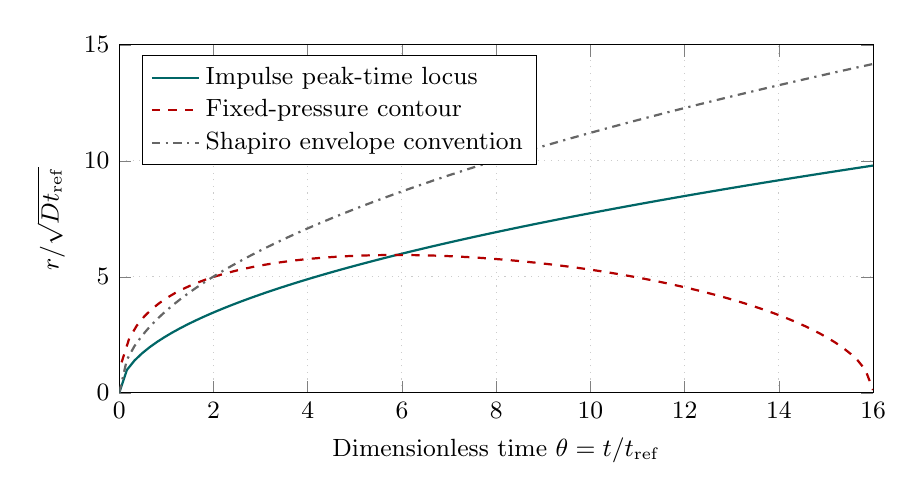
\begin{tikzpicture}
    \begin{axis}[width=0.92\linewidth, height=6cm,
        xlabel={Dimensionless time $\theta=t/t_{\mathrm{ref}}$},
        ylabel={$r/\sqrt{Dt_{\mathrm{ref}}}$}, xmin=0, xmax=16,
        ymin=0, ymax=15, grid=major, grid style={dotted,gray!40},
        font=\small, legend pos=north west, legend cell align=left,
      samples=100]
      \addplot[thick,teal!80!black,domain=0:16] {sqrt(6*x)};
      \addlegendentry{Impulse peak-time locus}
      \addplot[thick,red!70!black,dashed,domain=0.05:16]
      {sqrt(max(0,4*x*ln(64/(x^1.5))))};
      \addlegendentry{Fixed-pressure contour}
      \addplot[thick,black!60,dashdotted,domain=0:16] {sqrt(4*pi*x)};
      \addlegendentry{Shapiro envelope convention}
    \end{axis}
  \end{tikzpicture}
  \caption{Three distinct diffusion constructions: the impulse peak-time
    locus, a fixed-pressure contour, and the Shapiro envelope convention.
    Only the threshold contour retreats and terminates in this example.
    Curves are analytical illustrations with
    $Q_0/[S_{\mathrm s}p_*(4\pi Dt_{\mathrm{ref}})^{3/2}]=64$,
    $D,t_{\mathrm{ref}}>0$; no seismic catalogue is plotted and the
  envelope convention is not derived from the impulse threshold.}
  \label{fig:supp_diffusion_constructions}
\end{figure}

% ==============================================================================
% SECTION S5: INFORMATION THEORY, THERMODYNAMICS, AND UNIFIED GENERATIVE MODEL
% ==============================================================================
\subsection{Information Geometry, Field Theory, and the Unified
Generative Model}
\label{subsec:supp_info_thermo}

\paragraph{Derivation of the Landau Field Theory Critical Exponent
(\cref{eq:landau_functional,eq:critical_exponent}).}
The free energy functional governing temporal cluster order
parameter $\phi(t) \coloneqq \lambda(t) - \mu_0$ is:
\begin{equation}
  \mathcal{F}[\phi] \coloneqq \int_0^{T_{\mathrm{obs}}} \left[
    \frac{\kappa}{2}\,\dot{\phi}(t)^2
  + V(\phi; t) \right] \,\mathrm{d}t, \qquad \dot{\phi}(t) \equiv
  \frac{\mathrm{d}\phi}{\mathrm{d}t},
\end{equation}
where the potential density is:
\begin{equation}
  V(\phi; t) \coloneqq \frac{a(t)}{2}\phi^2 + \frac{c}{3}\phi^3 +
  \frac{b}{4}\phi^4,
\end{equation}
with $b > 0$, $\kappa > 0$, and $a(t) = a_0(t_c - t)$ with $a_0 > 0$.
The stationary states satisfy the Euler--Lagrange equation:
\begin{equation}
  \frac{\delta\mathcal{F}}{\delta\phi} = -\kappa \ddot{\phi}(t) +
  a(t)\phi + c\phi^2 + b\phi^3 = 0, \qquad \ddot{\phi}(t) \equiv
  \frac{\mathrm{d}^2\phi}{\mathrm{d}t^2}.
\end{equation}
For spatially and temporally slowly varying regimes (mean-field
approximation), neglect the acceleration term $\ddot{\phi} \approx 0$:
\begin{equation}
  \frac{\partial V}{\partial \phi} = \phi \bigl(a(t) + c\phi +
  b\phi^2\bigr) = 0.
\end{equation}
For continuous second-order transitions ($c = 0$), the stationary
solutions are:
\begin{equation}
  \phi = 0 \quad \text{or} \quad a(t) + b\phi^2 = 0 \implies \phi^2
  = -\frac{a(t)}{b}.
\end{equation}
For $t < t_c$, $a(t) = a_0(t_c - t) > 0$. The only real root is
$\phi^* = 0$, representing the disordered
(quiescent tectonic background) state with positive curvature
$V''(0) = a(t) > 0$.
For $t > t_c$, $a(t) = -a_0(t - t_c) < 0$. The state $\phi = 0$
becomes unstable ($V''(0) < 0$).
Spontaneous symmetry breaking creates two stable minima at:
\begin{equation}
  \phi_\pm^*(t) = \pm \sqrt{\frac{-a(t)}{b}} = \pm\sqrt{\frac{a_0(t -
  t_c)}{b}} \propto (t - t_c)^{1/2}, \qquad (t \ge t_c),
\end{equation}
giving the classical mean-field exponent $1/2$. Select the positive
branch for an enhanced rate; the negative branch is admissible only
while $\phi_-^*\ge-\mu_0$. This phenomenological construction does not
demonstrate a swarm critical exponent. For $c\ne0$, unconstrained
coexistence follows from $V(\phi)=V(0)$ and $V'(\phi)=0$, giving
$\phi=-2c/(3b)$ and $a=2c^2/(9b)$, subject again to the rate constraint.

\paragraph{Point-Process Kullback--Leibler and Jeffreys Divergences
(\cref{eq:pp_kl_divergence,eq:jeffreys_divergence}).}
Let $\mathbb{P}_A$ and $\mathbb{P}_B$ be probability measures
induced on the space of point trajectories
by predictable intensities $\lambda_A(t)$ and $\lambda_B(t)$.
The Radon--Nikodym derivative (likelihood ratio) is:
\begin{equation}
  \frac{\mathrm{d}\mathbb{P}_A}{\mathrm{d}\mathbb{P}_B} = \left(
  \prod_{i=1}^N \frac{\lambda_A(t_i)}{\lambda_B(t_i)} \right)
  \exp\left( -\int_0^{T_{\mathrm{obs}}} [\lambda_A(s) -
  \lambda_B(s)]\,\mathrm{d}s \right).
\end{equation}
The Kullback--Leibler divergence is defined as:
\begin{equation}
  \begin{aligned}
    \mathrm{D}_{\mathrm{KL}}(\mathbb{P}_A \parallel \mathbb{P}_B)
    &\coloneqq \mathbb{E}_A\left[ \ln
    \frac{\mathrm{d}\mathbb{P}_A}{\mathrm{d}\mathbb{P}_B} \right] \\
    &= \mathbb{E}_A\left[ \sum_{i=1}^N
      \ln\left(\frac{\lambda_A(t_i)}{\lambda_B(t_i)}\right) -
      \int_0^{T_{\mathrm{obs}}} [\lambda_A(s) -
    \lambda_B(s)]\,\mathrm{d}s \right].
  \end{aligned}
\end{equation}
First restrict to positive deterministic intensities with finite
divergence. By Campbell's theorem (\cref{eq:supp_campbell_mean}),
$\mathbb{E}_A[\sum_{i=1}^N g(t_i)] = \int_0^{T_{\mathrm{obs}}}
g(t)\lambda_A(t)\,\mathrm{d}t$.
Setting $g(t) = \ln(\lambda_A(t)/\lambda_B(t))$:
\begin{equation}
  \mathrm{D}_{\mathrm{KL}}(\mathbb{P}_A \parallel \mathbb{P}_B) =
  \int_0^{T_{\mathrm{obs}}} \lambda_A(t)
  \ln\left(\frac{\lambda_A(t)}{\lambda_B(t)}\right)\,\mathrm{d}t -
  \int_0^{T_{\mathrm{obs}}} \bigl[\lambda_A(t) -
  \lambda_B(t)\bigr]\,\mathrm{d}t,
\end{equation}
which proves \cref{eq:poisson_kl_explicit}. The symmetrized
Jeffreys divergence is:
\begin{equation}
  \begin{aligned}
    J(\lambda_A, \lambda_B) &\coloneqq
    \mathrm{D}_{\mathrm{KL}}(\lambda_A \parallel \lambda_B) +
    \mathrm{D}_{\mathrm{KL}}(\lambda_B \parallel \lambda_A) \\
    &= \int_0^{T_{\mathrm{obs}}} \left[
      \lambda_A(t)\ln\left(\frac{\lambda_A(t)}{\lambda_B(t)}\right) -
      (\lambda_A - \lambda_B) +
      \lambda_B(t)\ln\left(\frac{\lambda_B(t)}{\lambda_A(t)}\right) -
    (\lambda_B - \lambda_A) \right] \,\mathrm{d}t \\
    &= \int_0^{T_{\mathrm{obs}}} \left[
      \lambda_A(t)\ln\left(\frac{\lambda_A(t)}{\lambda_B(t)}\right) -
      \lambda_B(t)\ln\left(\frac{\lambda_A(t)}{\lambda_B(t)}\right)
    \right] \,\mathrm{d}t \\
    &= \int_0^{T_{\mathrm{obs}}} \bigl[\lambda_A(t) -
    \lambda_B(t)\bigr]
    \ln\left(\frac{\lambda_A(t)}{\lambda_B(t)}\right)\,\mathrm{d}t,
  \end{aligned}
\end{equation}
which is \cref{eq:jeffreys_divergence}. Since $(x - y)\ln(x/y)
\ge 0$ for all $x, y > 0$, $J(\lambda_A, \lambda_B) \ge 0$ identically,
giving a nonnegative statistical divergence, not a physical entropy
production rate. For predictable history-dependent intensities, retain
\begin{equation}
  D(P_A\parallel P_B)=\mathbb{E}_A\int_0^{T_{\mathrm{obs}}}
  \left[\lambda_A\ln\frac{\lambda_A}{\lambda_B}-\lambda_A+\lambda_B\right]
  \,\mathrm{d}t,
\end{equation}
under absolute continuity and integrability. The reverse divergence
uses $\mathbb{E}_B$, so the deterministic Jeffreys integral is not a
general formula for random conditional intensities.

\paragraph{Proof of Fisher--Rao Flatness in Log-Density Coordinates
(\cref{eq:fisher_metric_flat,eq:geodesic_distance}).}
Let $\rho>0$ be Poisson intensity per unit volume and $\rho_0>0$ a
reference intensity of the same units. The sampling experiment matters.
For a fixed observation volume $V>0$, the count $K\sim\mathrm{Poisson}(\rho V)$
has $\ell(\rho)=K\ln\rho-\rho V+\mathrm{const}$, giving
\begin{equation}
  g_{\rho\rho}=\frac{\mathbb{E}[K]}{\rho^2}=\frac{V}{\rho},\qquad
  g_{\phi\phi}=V\rho,\qquad \phi=\ln(\rho/\rho_0).
\end{equation}
Its constant-metric coordinate is $\xi=2\sqrt{V\rho}$, not $\phi$,
and $d_{\mathrm{FR}}=2\sqrt V\,|\sqrt{\rho_A}-\sqrt{\rho_B}|$.
For a fixed rank $k\ge1$, observe the stopping volume
$V_k\sim\mathrm{Gamma}(k,\text{rate }\rho)$. Now
$\ell(\rho)=k\ln\rho-\rho V_k+\mathrm{const}$, and
\begin{equation}
  g_{\rho\rho}=\frac{k}{\rho^2},\qquad
  g_{\phi\phi}=g_{\rho\rho}\left(\frac{\mathrm{d}\rho}{\mathrm{d}\phi}\right)^2=k.
  \label{eq:supp_metric_transformed}
\end{equation}
Consequently $\Gamma^\phi_{\phi\phi}=0$ for this experiment, its
geodesics are $\phi(s)=(1-s)\phi_A+s\phi_B$, $s\in[0,1]$, and
\begin{equation}
  d_{\mathrm{FR}}(\rho_A,\rho_B)
  =\sqrt{k}\,|\ln(\rho_A/\rho_B)|.
\end{equation}
This proves \cref{thm:fisher_rao_flatness} for the same fixed $k$ at
both endpoints. One-dimensional curvature vanishes in either experiment;
it does not by itself identify the constant-metric coordinate.

\begin{figure}[htbp]
  \centering
  \begin{tikzpicture}
    \node[clusteringTheory,text width=0.84\linewidth] (volume)
    {Fixed volume $V$: random count $K\sim\mathrm{Poisson}(\rho V)$\\
    $g_{\rho\rho}=V/\rho$; constant coordinate $2\sqrt{V\rho}$};
    \node[clusteringTheory,text width=0.84\linewidth,below=4mm of
    volume] (rank)
    {Fixed rank $k$: random volume $V_k\sim\mathrm{Gamma}(k,\rho)$\\
    $g_{\rho\rho}=k/\rho^2$; constant coordinate $\sqrt{k}\ln(\rho/\rho_0)$};
    \node[clusteringImpl,text width=0.84\linewidth,below=4mm of
    rank] (adaptive)
    {Adaptive PAk: $k^*$ selected from the neighbourhood data\\
    Fixed-rank Gamma and coverage identities need separate justification};
  \end{tikzpicture}
  \caption{Sampling experiments underlying density uncertainty and Fisher
    geometry. Fixing exposure or rank produces different metrics; adaptive
    rank selection is not a third exact Gamma identity. Dashed boxes show
    ideal homogeneous Poisson experiments; the solid box identifies the
    selection implemented in \texttt{OGS/src/ogsclustering.py}, without a
  claim of selection-aware statistical calibration.}
  \label{fig:supp_sampling_experiments}
\end{figure}

\paragraph{Analytical Integration of the Unified Compensator
(\cref{eq:analytical_compensator}).}
The unified conditional intensity
(\cref{eq:unified_conditional_intensity}) is:
\begin{equation}
  \lambda(t \mid \mathcal{H}_t) = \mu_0(t) + \sum_{k=1}^K A_k
  \phi_k(t) + \sum_{t_j < t} \kappa(m_j)\psi(t - t_j).
\end{equation}
The total compensator on $[0, T_{\mathrm{obs}}]$ is
$\Lambda(T_{\mathrm{obs}}) = \int_0^{T_{\mathrm{obs}}} \lambda(s
\mid \mathcal{H}_s)\,\mathrm{d}s$.
Integrating term by term:
\begin{enumerate}
  \item Background term: For piecewise-constant $\mu_0(t) =
    \sum_{j=0}^J \mu_j \mathbf{1}_{(\tau_j, \tau_{j+1}]}(t)$:
    \begin{equation}
      \int_0^{T_{\mathrm{obs}}} \mu_0(s)\,\mathrm{d}s = \sum_{j=0}^J
      \mu_j (\tau_{j+1} - \tau_j).
    \end{equation}
  \item Swarm envelope term: Assume $0\le t_0^{(k)}<T_{\mathrm{obs}}$
    and a fixed time unit. For log-normal pulse $\phi_k(t)$:
    \begin{equation}
      \phi_k(t) = \frac{1}{(t -
      t_0^{(k)})\sigma_k\sqrt{2\pi}}\exp\left(-\frac{(\ln(t -
            t_0^{(k)}) -
      \nu_k)^2}{2\sigma_k^2}\right)\mathbf{1}_{(t_0^{(k)}, \infty)}(t).
    \end{equation}
    Substituting $u = \ln(s - t_0^{(k)})$, $\mathrm{d}u =
    \frac{\mathrm{d}s}{s - t_0^{(k)}}$:
    \begin{equation}
      \begin{aligned}
        \int_0^{T_{\mathrm{obs}}} \phi_k(s)\,\mathrm{d}s
        &=\int_{-\infty}^{\ln(T_{\mathrm{obs}}-t_0^{(k)})}
        \frac{e^{-(u-\nu_k)^2/(2\sigma_k^2)}}{\sigma_k\sqrt{2\pi}}
        \,\mathrm{d}u \\
        &=\Phi\left(\frac{\ln(T_{\mathrm{obs}}-t_0^{(k)})-\nu_k}{\sigma_k}\right)
        \\
        &\equiv\Phi_{\mathrm{LN}}\bigl(\ln(T_{\mathrm{obs}}-t_0^{(k)});
        \,\nu_k,\sigma_k\bigr).
      \end{aligned}
    \end{equation}
  \item Triggered aftershock cascades: Assume empty pre-observation history.
    For Omori kernel $\psi(\tau)
    = \frac{(p - 1)c^{p-1}}{(\tau + c)^p}$:
    \begin{equation}
      \begin{aligned}
        \int_0^{T_{\mathrm{obs}}} \left(\sum_{j: t_j < s}
        \kappa(m_j)\psi(s - t_j)\right)\mathrm{d}s
        &= \sum_{j=1}^N \kappa(m_j) \int_{t_j}^{T_{\mathrm{obs}}}
        \psi(s - t_j)\,\mathrm{d}s \\
        &= \sum_{j=1}^N \kappa(m_j) \int_0^{T_{\mathrm{obs}} - t_j}
        \frac{(p - 1)c^{p-1}}{(u + c)^p}\,\mathrm{d}u \\
        &= \sum_{j=1}^N \kappa(m_j) (p - 1)c^{p-1} \left[ -\frac{(u
        + c)^{1-p}}{p - 1} \right]_0^{T_{\mathrm{obs}} - t_j} \\
        &= \sum_{j=1}^N \kappa(m_j) c^{p-1} \left[ c^{1-p} -
        (T_{\mathrm{obs}} - t_j + c)^{1-p} \right] \\
        &= \sum_{j=1}^N \kappa(m_j) \left[ 1 - \left(
        \frac{c}{T_{\mathrm{obs}} - t_j + c} \right)^{\!p-1} \right].
      \end{aligned}
    \end{equation}
\end{enumerate}
Summing gives \cref{eq:analytical_compensator} under these onset and
history restrictions. For general onset $t_0$, define the shifted-delay
CDF $F_{\mathrm{LN}}(x)=0$ for $x\le0$ and
$F_{\mathrm{LN}}(x)=\Phi[(\ln x-\nu)/\sigma]$ for $x>0$.
The pulse integral is then $F_{\mathrm{LN}}(T_{\mathrm{obs}}-t_0)
-F_{\mathrm{LN}}(-t_0)$. Pre-observation parents likewise require
lower-limit subtraction; $\Phi$ denotes the standard normal CDF.

\paragraph{Three-Way Stochastic Declustering Normalization
(\cref{eq:three_way_responsibilities}).}
At event time $t_i$, the conditional intensity decomposes as:
\begin{equation}
  \lambda(t_i \mid \mathcal{H}_{t_i}) = \mu_0(t_i) + \sum_{k=1}^K
  A_k \phi_k(t_i) + \sum_{t_j < t_i} \kappa(m_j)\psi(t_i - t_j).
\end{equation}
Defining the three posterior responsibilities:
\begin{equation}
  w_i^{(\mathrm{bg})} \coloneqq \frac{\mu_0(t_i)}{\lambda(t_i)}, \qquad
  w_i^{(\mathrm{env}, k)} \coloneqq \frac{A_k
  \phi_k(t_i)}{\lambda(t_i)}, \qquad
  w_i^{(\mathrm{trig})} \coloneqq \frac{\sum_{t_j <
  t_i}\kappa(m_j)\psi(t_i - t_j)}{\lambda(t_i)}.
\end{equation}
Summing across all components:
\begin{equation}
  w_i^{(\mathrm{bg})} + \sum_{k=1}^K w_i^{(\mathrm{env}, k)} +
  w_i^{(\mathrm{trig})}
  = \frac{\mu_0(t_i) + \sum_{k=1}^K A_k \phi_k(t_i) + \sum_{t_j <
  t_i}\kappa(m_j)\psi(t_i - t_j)}{\lambda(t_i \mid
  \mathcal{H}_{t_i})} \equiv 1,
\end{equation}
giving normalized component responsibilities when all contributions are
nonnegative and $\lambda(t_i)>0$. Normalization does not establish the
physical origin of an event or identifiability of the fitted components.

% ==============================================================================
% SECTION S6: VECTORIZED ADVANCED DENSITY PEAKS (ADP++)
% ==============================================================================
\subsection{Vectorized ADP++ Complexity and Pointer Jumping Convergence}
\label{subsec:supp_adppp_vectorized}

\paragraph{Convergence of Parallel Pointer Jumping
(\cref{thm:union_find_equivalence}).}
Let $\mathcal{G}_{\mathrm{ascent}} = (\mathcal{V}, \mathcal{E})$ be
the directed graph
with vertices $\mathcal{V} = \{1, \dots, N\}$ and edges $(i, p_i)$
defined by the parent link array:
\begin{equation}
  p_i \coloneqq \argmax_{j \in \mathcal{N}_i^{\kstar(i)},\; g_j >
  g_i} g_j, \qquad (\text{with } p_i = i \text{ if } \max_{j} g_j \le g_i).
\end{equation}
Because an edge $(i, p_i)$ with $p_i \ne i$ strictly increases the
score ($g_{p_i} > g_i$),
no directed cycles can exist. Thus $\mathcal{G}_{\mathrm{ascent}}$
is a directed forest
rooted at the local peaks $\mathcal{P} = \{k \in \mathcal{V} : p_k = k\}$.
Pointer jumping updates the array via:
\begin{equation}
  \mathbf{r}^{(0)} = \mathbf{p}, \qquad \mathbf{r}^{(t+1)} =
  \mathbf{r}^{(t)}\bigl[\mathbf{r}^{(t)}\bigr].
\end{equation}
We prove by induction that after iteration $t$,
$\mathbf{r}^{(t)}[i]$ points to the ancestor
at distance $\min(2^t, L(i))$ from node $i$, where $L(i)$ is the
path length from $i$ to its root peak $c(i)$.
\begin{itemize}
  \item \textbf{Base Case ($t = 0$):} $\mathbf{r}^{(0)}[i] = p_i$,
    which is at distance $1 = 2^0$ (or $0$ if $i$ is a root).
  \item \textbf{Inductive Step:} Assume $\mathbf{r}^{(t)}[i]$ is at
    distance $\min(2^t, L(i))$. Then:
    \begin{equation}
      \mathbf{r}^{(t+1)}[i] = \mathbf{r}^{(t)}\bigl[\mathbf{r}^{(t)}[i]\bigr].
    \end{equation}
    If $2^t \ge L(i)$, then $\mathbf{r}^{(t)}[i] = c(i)$. Since
    $c(i)$ is a root, $\mathbf{r}^{(t)}[c(i)] = c(i)$, so
    $\mathbf{r}^{(t+1)}[i] = c(i)$.
    If $2^t < L(i)$, let $j = \mathbf{r}^{(t)}[i]$ be the ancestor
    at distance $2^t$.
    By induction hypothesis applied to node $j$,
    $\mathbf{r}^{(t)}[j]$ points to the ancestor at distance
    $\min(2^t, L(j))$ from $j$.
    The total distance from $i$ is $2^t + \min(2^t, L(i) - 2^t) =
    \min(2^{t+1}, L(i))$.
\end{itemize}
Let $L_{\max} = \max_{i} L(i)$ be the maximum path length.
When $2^t \ge L_{\max}$, every node points directly to its peak root:
\begin{equation}
  t^* = \left\lceil\log_2\max(1,L_{\max})\right\rceil
  \le \lceil \log_2 N \rceil,
\end{equation}
giving zero required updates when every pointer already reaches a root.
Each array update costs $\mathcal{O}(N)$ work, so total work is
$\mathcal{O}(N[1+\log\max(1,L_{\max})])$, with potentially an extra
termination check. Equivalence is to sequential traversal of the
\emph{same parent forest}; scalar ADP's centre pruning and tie handling
do not generally construct that forest.

\begin{figure}[htbp]
  \centering
  \begin{tikzpicture}
    \node[clusteringImpl,text width=0.78\linewidth] (initial)
    {Chain $1\to2\to3\to4\to5$; $5$ is a root\\
    $\mathbf r^{(0)}=(2,3,4,5,5)$: reach $1$ edge};
    \node[clusteringImpl,text width=0.78\linewidth,below=7mm of
    initial] (second)
    {$\mathbf r^{(1)}=(3,4,5,5,5)$: reach up to $2$ edges};
    \node[clusteringImpl,text width=0.78\linewidth,below=7mm of
    second] (fourth)
    {$\mathbf r^{(2)}=(5,5,5,5,5)$: reach up to $4$ edges};
    \draw[clusteringArrow] (initial) -- (second);
    \draw[clusteringArrow] (second) -- (fourth);
  \end{tikzpicture}
  \caption{Pointer jumping on an illustrative five-node ascent chain.
    Ancestor reach doubles at each update until all pointers reach root~5;
    an all-root input needs no updates. Solid boxes illustrate the array
    operation in \texttt{OGS/src/ogsclustering.py}; the convergence proof
    concerns this fixed forest, not universal parity with scalar ADP.
  Parallel rounds and total array work are different complexity measures.}
  \label{fig:supp_pointer_jumping}
\end{figure}

\paragraph{Vectorized Border First-Hit Equivalence
(\cref{eq:border_tensor,eq:vectorized_first_hit}).}
In scalar ADP, border points are identified by iterating
sequentially over sorted neighbours
$j \in \mathcal{N}_i$: the algorithm breaks at the first neighbour
$j$ with cluster label $C_j \ne \ell_i$.
In \textsc{ADP++}, the boolean border tensor is:
\begin{equation}
  B_{ij} = \mathbf{1}_{\{C_{\mathrm{nb}, ij} \ne \ell_i\}} \cdot
  \mathbf{1}_{\{j \le \kstar(i)\}}.
\end{equation}
The vectorized first-hit index is evaluated via:
\begin{equation}
  j_{\mathrm{first}}(i) = \argmax_{j \in \{1, \dots, k_{\max}\}} B_{ij}.
\end{equation}
Apply this index only when $h_i=\max_jB_{ij}=1$.
In standard NumPy semantics, \texttt{argmax} along a boolean axis
returns the index
of the first occurrence of \texttt{True} (value 1). If all elements are
\texttt{False}, a zero-based implementation returns 0, which must not
be interpreted as a border. The inspected implementation includes this
guard. This establishes first-hit equivalence for identical neighbour
orderings and labels, not bitwise parity of every subsequent tied reduction.

% ==============================================================================
% SECTION S7: TOPOLOGICAL CLUSTER VALIDITY VIA PAK-DS SCORE
% ==============================================================================
\subsection{PAk Density Separation Score and Morse Persistence}
\label{subsec:supp_ds_score}

\paragraph{Pairwise Density Separation Score Formulations
(\cref{eq:pairwise_zscore,eq:pairwise_zscore_robust}).}
Let clusters $C_c, C_{c'}$ have peak log-densities $\hat{u}_c,
\hat{u}_{c'}$ with uncertainties
$\hat{\sigma}_c, \hat{\sigma}_{c'}$, and saddle log-density
$\hat{u}_{cc'}^\dagger$ with uncertainty $\hat{\sigma}_{cc'}^\dagger$.
The density contrast between the shallower peak and the saddle is:
\begin{equation}
  \Delta \hat{u}_{cc'} \coloneqq \min(\hat{u}_c, \hat{u}_{c'}) -
  \hat{u}_{cc'}^\dagger.
\end{equation}
The general variance identity includes covariance:
\begin{equation}
  \Var\bigl(\Delta \hat{u}_{cc'}\bigr) = \Var\bigl(\min(\hat{u}_c,
  \hat{u}_{c'})\bigr) + \Var\bigl(\hat{u}_{cc'}^\dagger\bigr)
  -2\Cov\bigl(\min(\hat u_c,\hat u_{c'}),\hat u_{cc'}^\dagger\bigr).
\end{equation}
For well-separated peak values $|\hat{u}_c - \hat{u}_{c'}| \gg
\sqrt{\hat{\sigma}_c^2 + \hat{\sigma}_{c'}^2}$,
the minimum is dominated by the lower peak $c_{\min} =
\argmin(\hat{u}_c, \hat{u}_{c'})$:
\begin{equation}
  \Var\bigl(\min(\hat{u}_c, \hat{u}_{c'})\bigr) \approx
  \hat{\sigma}_{\min(c, c')}^2.
\end{equation}
If the lower peak is prespecified and independent of the saddle, the
plug-in variance approximation is $\sigma_{\mathrm{total}}^2 =
\hat{\sigma}_{\min(c, c')}^2 + (\hat{\sigma}_{cc'}^\dagger)^2$.
The corresponding lower-peak-only alternative is:
\begin{equation}
  Z_{cc'}^{(\mathrm{lower})} = \frac{\Delta
  \hat{u}_{cc'}}{\sigma_{\mathrm{total}}}
  = \frac{\min(\hat{u}_c, \hat{u}_{c'}) -
  \hat{u}_{cc'}^\dagger}{\sqrt{\hat{\sigma}_{\min(c, c')}^2 +
  (\hat{\sigma}_{cc'}^\dagger)^2}},
\end{equation}
which is \cref{eq:pairwise_zscore_robust}, not the operational score.
The inspected code uses both peak errors in \cref{eq:pairwise_zscore},
with a saddle error obtained from its selected border edge. Shared
neighbours, nearly tied peaks, and extremum selection invalidate a
general independent-normal interpretation of either denominator.

\paragraph{0-Homology Persistence and the Limits of Calibration
(\cref{eq:calibrated_persistence,eq:zscore_pvalue}).}
In Morse theory, the superlevel filtration $L(\lambda) =
\{\mathbf{x} : f(\mathbf{x}) \ge \lambda\}$
generates 0-dimensional homology classes (connected components).
A connected component is born at a local maximum with birth value
$b_c = f(\mathbf{x}_c)$.
On a $d$-dimensional manifold, component-merging saddles of $f$ have
Morse index $d-1$; maxima have index $d$. Indices 0 and 1 instead
refer to $-f$. Two components merge with death value $d_{cc'}
= f(\mathbf{x}_{cc'}^\dagger)$.
By the Elder rule of persistent homology:
\begin{itemize}
  \item The component with the higher birth value
    ($b_{\mathrm{elder}} = \max(b_c, b_{c'})$) survives the merge.
  \item The component with the lower birth value
    ($b_{\mathrm{younger}} = \min(b_c, b_{c'})$) dies at $d_{cc'}$.
\end{itemize}
The topological persistence of the dying component is:
\begin{equation}
  \pi_{cc'} \coloneqq b_{\mathrm{younger}} - d_{cc'} = \min(b_c,
  b_{c'}) - d_{cc'}.
\end{equation}
For positive density values, a log transform preserves pairings but
changes lifetime to $\pi_u=\ln b_{\mathrm{younger}}-\ln d_{cc'}$.
Empirical border estimates are discrete proxies, not automatically
critical points of a Morse function. For a prespecified contrast with
consistent standard-error estimate $\hat\sigma$ and an independently
justified central limit theorem, a boundary-null test would use
$Z=\hat\pi_u/\hat\sigma$. Its nominal one-sided normal tail is:
\begin{equation}
  p_{\mathrm{nom}} = 1 - \Phi(Z) =
  \frac{1}{\sqrt{2\pi}}\int_Z^\infty e^{-t^2/2}\,\mathrm{d}t
  = \frac{1}{2}\operatorname{erfc}\left(\frac{Z}{\sqrt{2}}\right).
\end{equation}
Setting $Z_{\mathrm{crit}} \coloneqq \num{3.0}$ corresponds to:
\begin{equation}
  p = 1 - \Phi(\num{3.0}) \approx \num{1.3499e-3},
\end{equation}
The two-sided tail is approximately $\num{2.6998e-3}$.
These are reference probabilities, not calibrated PAk-DS $p$-values.
Selection of maxima, saddles, and ranks can produce positive contrasts
under unimodality. False-discovery control requires valid selection-aware
$p$-values and an explicit multiplicity procedure, neither established here.

\begin{figure}[htbp]
  \centering
  \begin{tikzpicture}
    \node[clusteringTheory,text width=38mm] (elder)
    {Higher peak\\birth $b_{\mathrm e}$};
    \node[clusteringTheory,text width=38mm,right=12mm of
    elder,yshift=-9mm] (younger)
    {Lower peak\\birth $b_{\mathrm y}$};
    \node[clusteringTheory,text width=48mm,below=22mm of
    elder,xshift=26mm] (saddle)
    {Connecting saddle $d$\\younger component dies};
    \node[clusteringTheory,text width=48mm,below=8mm of saddle] (survivor)
    {Older component survives};
    \draw[clusteringArrow] (elder.south) -- (saddle.north west);
    \draw[clusteringArrow] (younger.south) -- (saddle.north east);
    \draw[clusteringArrow] (saddle) -- (survivor);
  \end{tikzpicture}
  \caption{Elder-rule pairing in a superlevel filtration of a positive
    Morse density as the threshold descends. The younger component dies
    at the connecting saddle: raw lifetime is $b_{\mathrm y}-d$, whereas
    log-density lifetime is $\ln(b_{\mathrm y}/d)$, with $b_{\mathrm e}
    \ge b_{\mathrm y}>d>0$. Dashed boxes denote a theoretical schematic,
  not sampled Morse critical points or calibrated statistical tests.}
  \label{fig:supp_persistence_pairing}
\end{figure}

\paragraph{Kramers Escape Time as a Conditional Physical Analogy
(\cref{eq:kramers_time}).}
For a one-dimensional overdamped diffusion in a smooth energy potential
$U$, let $\mu_{\mathrm{mob}}>0$ be mobility, $\epsilon=k_{\mathrm B}T>0$
the noise energy scale, and $W_t$ standard Brownian motion:
\begin{equation}
  \mathrm{d}X_t=-\mu_{\mathrm{mob}}U'(X_t)\,\mathrm{d}t
  +\sqrt{2\mu_{\mathrm{mob}}\epsilon}\,\mathrm{d}W_t.
\end{equation}
For a nondegenerate well at $x_a$ and intervening barrier at $x_s$,
with $U''(x_a)>0$, $U''(x_s)<0$, and
$\Delta U=U(x_s)-U(x_a)\gg\epsilon$, the inter-well Kramers time is
\begin{equation}
  \tau\sim\frac{2\pi}{\mu_{\mathrm{mob}}
  \sqrt{U''(x_a)|U''(x_s)|}}\exp(\Delta U/\epsilon).
\end{equation}
If one additionally postulates $U=-E_0\ln(\rho/\rho_0)$ with
$E_0>0$ an energy scale, then $\Delta U=E_0\ln(\rho_a/\rho_s)$
and \cref{eq:kramers_time} follows with $\beta=E_0/\epsilon$.
PAk uncertainty is not $\epsilon$, and the source code specifies no
such stochastic dynamics, mobility, or physical energy scale.
Therefore a large separation score alone implies neither a physical
escape time nor a long-lived thermodynamic state.
